\documentclass[12pt]{article}
\usepackage[utf8]{inputenc}
\usepackage{graphicx} % Allows you to insert figures
\usepackage{amsmath} % Allows you to do equations
\usepackage{fancyhdr} % Formats the header
\usepackage{geometry} % Formats the paper size, orientation, and margins
\setlength{\parindent}{0pt} % no paragraph indents
\setlength{\parskip}{1em} % paragraphs separated by one line
\usepackage[format=plain,
            font=it]{caption} % Italicizes figure captions
\usepackage[english]{babel}
\usepackage{csquotes}
\renewcommand{\headrulewidth}{0pt}
\geometry{letterpaper, portrait, margin=1in}
\setlength{\headheight}{14.49998pt}
\usepackage{mathtools}
\usepackage[normalem]{ulem}
\usepackage{caption}
\usepackage{subcaption}
\usepackage{cite}
\usepackage{nicefrac}
\usepackage{wrapfig}
\usepackage{hyperref}
\usepackage[all]{xy}
\usepackage{qcircuit}
\usepackage{amsthm}
\usepackage{physics}
\usepackage{url}
\usepackage{hyperref}
\usepackage{filecontents}
\usepackage[backend=bibtex]{biblatex}
\usepackage{xcolor}
\usepackage{unicode-math}
\usepackage{tabularray}
\usepackage{bbm}
\usepackage{makecell}
\usepackage{booktabs}
\usepackage{amsfonts}
\addbibresource{./qiskit.bib}
\numberwithin{equation}{section}
\ One defines usepackage{amsmath}
\usepackage{amssymb}
\newtheorem{prettytheorem}{Theorem}[section]
\usepackage{framed}
\usepackage{minted}


\begin{document}


 \begin{center}

\hspace{5cm}
   \vspace{5cm}

 \Huge{Notes on basic notions of basic Quantum algorithms} 
 \vspace{1cm}
\\ \huge A mathematical perspective\\ 

\hspace{10pt}

% Author names and affiliations
\large
Leo Kruglikov
\vspace{0.5cm}


\today

\hspace{10pt}

%\small  
%$^1$) First affiliation\\
%arthur.author@correspondence.email.com\\
%$^2$) Second affiliation

\end{center}

\hspace{10pt}

\normalsize

%This is a simple one-page abstract template. Please keep your abstract length at one page. The abstract should be in English. You may include figures and pictures in your abstract, as long as they fit in the single page limit.

%Sed ut perspiciatis unde omnis iste natus error sit voluptatem accusant
\newcommand{\qvdots}{% \vdots for qcircuit
  \raisebox{0.3em}{\ensuremath{\vdots}}%
}

\newpage

\tableofcontents

\theoremstyle{concept}
\newtheorem{concept}{Concept}[section]




\section{Concepts and notions}

\subsection*{Fundamentals}
\paragraph{} Here I non-rigourously describe the main notions that are used during the algorithm discussions.
\begin{concept}
  A quantum cirquit is composed of a (multiple) qubit(s) input and a measurable output of the same size.
  If multiple qubits are involved, the inputs are mathematically defined: 
  \begin{gather}
    \text{input of n qubits }\ket{\psi_i} = \bigotimes_{i=1}^{n}\ket{\psi_i}
  \end{gather}
\end{concept}

\begin{concept}
  A quantum circuit is composed of different and various gates, that can be applied on multiple qubits. Every gate is an operator.
  If a gate $\widehat{O}$ is applied only on state $\ket{\psi_i}$, the operator on the whole system is given by 
  \begin{gather}
    \widehat{O}_{\text{on state i}} = \mathbbm{1}_{(1)}\otimes \mathbbm{1}_{(2)}\otimess \cdots \otimes \mathbbm{1}_{(i-1)}\otimes 
    \widehat{O}\otimes \mathbbm{1}_{(i+1)} \cdots \otimes \mathbbm{1}_{(n)}
  \end{gather}
\end{concept}
%\begin{concept}[Quantum function evaluation]
%Consider some kind of quantum cirquit and a function. I define the \textsl{(basic)} quantum function evaluation by the circuit given below:
%\end{concept}
%
%
%\begin{figure}[ht!]
%  \Qcircuit @C=1em @R=1em{
%    \lstick{\ket{0}} & \qw & \multigate{1}{U} & \qw \\
%    \lstick{\ket{0}} & \qw & \ghost{U} & \qw \\
%    \lstick{\ket{0}} & \qw & \ghost{U} & \qw \\
%  }
%  \label{fig:function_evaluation}
%\caption{Quantum function evaluation.}
%\end{figure}
%
%What the binary algorithm does is to \textsl{evaluate the function of the target cubit}.

\subsection*{Main Circuits}
Let's discuss main representation of the circuits.

\begin{table}[ht!]
  \begin{tabular}{|c|c|c|c|c|}
    \hline
    Operator & \makecell{Bra-Ket \\ representation} & Matrix & \makecell{Other math \\ properties} & Qiskit \\
    \hline 
    \hline
    \makecell{Identity op. \\ $I=\text{Id}=\mathbbm{1}$}  & \makecell{Closure relation: \\ $\forall \{a_i\}\in V$ \\ $\mathbbm{1}=\sum_i \ket{v_i}\bra{v_i}$ } & $\begin{bmatrix} 1 & 0 \\ 0 & 1 \end{bmatrix}$ & $\forall \ket{\psi} \in V , \mathbbm{1}\ket{\psi}=\ket{\psi}$ &  \\
    \hline
    \makecell{Hadamard op. \\ $H=\mathcal{H}$ } & \makecell{In the $Z/X$ basis \\ $\mathcal{H}=\ket{+}\bra{0} + \ket{-}\bra{1}$} &
    $\frac{1}{\sqrt{2}}\begin{bmatrix} 1 & 1 \\ 1 & -1 \end{bmatrix}$ & \makecell{Change of basis from \\ $Z$ to $X$ basis.} & \\
    \hline 
    \makecell{Z-gate \\ $\sigma_z = Z$} & $\sigma_z \equiv \ket{0}\bra{1} - \ket{1}\bra{1}$ & $ \begin{bmatrix} 1 & 0 \\ 0 & -1 \end{bmatrix} $ &
    \makecell{Eigen-op. of the \\ $\ket{+1;\hat{S}_z}=\ket{0}$ state} & \\
    \hline
    \makecell{X-gate \\ $\sigma_x = X$} & \makecell{$\sigma_x \equiv \ket{0}\bra{1}+\ket{1}\bra{0}$ \\ $\sigma_x \equiv \ket{+}\bra{+} - \ket{-}\bra{-}$ } & $\begin{bmatrix} 0 & 1 \\ 1 & 0 \end{bmatrix}$ & 
    \makecell{Eigen-op. of the \\ $\ket{+}\equiv \frac{1}{\sqrt{2}}(\ket{0}+\ket{1})$} & \\
\hline
    \makecell{phase gate\\ $P(\phi)$} & $P(\phi)\equiv \ket{0}\bra{0} + e^{i\phi}\ket{1}\ket{1}$ & $\begin{bmatrix} 1&0\\0&e^{i\phi} \end{bmatrix}$ & & \\
    \hline
    \makecell{Controlled-NOT \\
      \Qcircuit @C=1em @R=0.5em{
    \qw & \ctrlo{1}&\qw\\
    \qw & \targ & \qw
    }
  }& \makecell{
  $\text{CNOT}=\\=\ket{0}\bra{0}\otimes \mathbbm{1}+\ket{1}\bra{1}\otimes X$\\
  \ket{x_{c}}\ket{x_{t}}\xrightarrow{CNOT} \ket{x_{c}}\ket{x_{c}\oplus x_{t}}
  } & 
  $\begin{bmatrix}
    1&0&0&0\\
    0&1&0&0\\
    0&0&0&1\\
    0&0&1&0
  \end{bmatrix}$ &
  \makecell{Acting on a 4x1 vec.\\spanned by \\$\{\ket{00},\ket{01},\ket{10},\ket{11}\} } 
  & \\
  \hline
  \end{tabular}    
\end{table}

\subsection*{Inner product}
\label{subsec:inner_product}
One have seen the importance of the inner/dot product of two kets in quantum mechanics.
Namely, how to evaluate a bra-ket of two states $\ket{a}$ and $\ket{b}$ - $|\bra{a}\ket{b}|^2$.
For that, one prepares a state $\ket{a}\ket{b}$ together with a helper qubit $\ket{0}$.
The resulting state will therefore be $\ket{0}\ket{a}\ket{b}$.

One then applies the Hadamard gate to the first qubit $\ket{0}$, yielding the state $\nicefrac{1}{\sqrt{2}}(\ket{0}+\ket{1})\ket{a}\ket{b}$.
One then applies a controlled-swap operator on the last 2 qubits $\ket{a}\ket{b}$. 
The controlled swap operator is an operator that swaps 2 qubits if the controlled qubit is $\ket{1}$. 
The result is therefore given by $\nicefrac{1}{\sqrt{2}}(\ket{0}\ket{a}\ket{b}+\ket{1}\ket{b}\ket{a})$. Finally, one applies 
the Hadamard gate on the first qubit:
\begin{equation}
  \begin{split}
  \mathcal{H}\otimes\mathbbm{1}\otimes \mathbbm{1}  \frac{1}{\sqrt{2}}\Biggl(\ket{0}\ket{a}\ket{b}+\ket{1}\ket{b}\ket{a}\Biggr) = 
  \frac{1}{2}(\ket{0}+\ket{1})\ket{a}\ket{b} + \frac{1}{2}(\ket{0}-\ket{1})\ket{b}\ket{a} = \\
  = \frac{1}{2}\Biggl( \ket{0}(\ket{a}\ket{b}+\ket{b}\ket{a}) + \ket{1}(\ket{a}\ket{b}-\ket{b}\ket{a})\Biggr) \equiv \ket{\psi}
\end{split}
\end{equation}
Now, one can finally measure the obtained state. Thus one asks the question on the probability of measuring the 
state $\ket{0}$. The probability is therefore is given by $|\bra{\bra{0}\otimes \mathbbm{1}\otimes \mathbbm{1}}\ket{\psi}|^2$.
It is easy to verify that this probability is given by 
\begin{equation}
  p_{\ket{0}} = \frac{1}{2} - \frac{1}{2}|\bra{a}\ket{b}|^2
\end{equation}
This can be evaluated by multiple shots of the algorithm.












\newpage

\theoremstyle{definition}
\newtheorem{definition}{Definition}[section]

\section{Deutsch-Jozsa algorithm}
The Deutsch-Jozsa algorithm was the first algorithm to be proposed.
The goal of the Deutsch's quantum algorithm is to determine a concrete property of a funciton. In this case, we use the quantum 
algorithm, to determine the properties of the function. In the case of the 
\begin{definition}[Constant and balanced]
  The function used here is a function from $\{0,1\}^N \mapsto \{0,1\}$. The outputs of it can be either constant or balanced.
  We say that the function is \textit{constant} if for \underline{any} input the output is constant, that is, whether all ones or all zeroes.
  We say that the function is \textit{balanced} if it outputs ones half of the times and zeroes half of the other times (that is, out of all 
possible inputs, it will output a \verb|1| in the half of the input cases and \verb|0| in the other).
\end{definition}
We will consider the case where $n$ (the number of inputs) is equal to one. That is, the function $f(x)$ has one input bit. $f(x)$, with $x \in \{0,1\}$.
Let's see examples of functions that are either balanced or constant. Let $f_1(x)$. The function happens to output the following: $f_1(0)=0$ and $f_1(1)=0$. We see that the 
function has zeroes for any input. Therefore, we can conclude that the function $f_1$ is constant. Consider now the function $f_2$, satisfying the following:
$f_2(0)=1$ and $f_2(1)=0$. As there are 2 kinds of inputs (\verb|0| and \verb|1|), there are only 2 possible outputs (2 different outputs for 2 different inputs).
We see that for the function $f_2$, half of the outputs (i.e. only one out of two) is \verb|0| and half of the inputs is \verb|1|. Therefore, the function $f_2$ is 
balanced.

The example was a simple case, where the input was simply either \verb|0| or \verb|1|. The definition of this constant/balanced can be extended to a more complex case 
of an input $\{0,1\}^n$, which is the Deutsch-Jozsa algorithm. 
\subsection*{Deutsch's algorithm}
Let's first consider the Deutsch's algorithm \cite{noauthor_deutschjozsa_2022}, that is, with one input bit. Note that in this algorithm we assume or we are promised that the given function is either balanced or constant (it can be neither). The circuit is \textit{postulated} to be.
In order for it to have a working mechanism, we need to prepare the initial states.


\begin{figure}[ht!]
     \begin{subfigure}[b]{0.4\textwidth}
\Qcircuit @C=1em @R=1em{
  \qw & \gate{\mathcal{H}} & \ctrl{1} & \gate{\mathcal{H}} & \qw \\
  \qw & \qw      & \gate{f} & \qw      & \qw \\
}
\caption{Deutsch's circuit}
     \end{subfigure}
     \hfill
     \begin{subfigure}[b]{0.4\textwidth}
\hspace{1cm}
\Qcircuit @C=1em @R=1em{
  \lstick{\ket{0}}           & \qw & \gate{\mathcal{H}}& \ustick{A}\qw  & \ctrl{1} &\ustick{B}\qw & \gate{\mathcal{H}} & \qw \\
  \lstick{\ket{0} - \ket{1}} & \qw & \qw     &\ustick{A}\qw   & \gate{f} & \qw          &\qw      & \qw \\
}

\caption{Initialized states}
     \end{subfigure}
  \caption{Deutsch's circuit}
  \label{cirq:deutsch_start}

\end{figure}

Having the circuit with prepared initial states (\autoref{cirq:deutsch_start}) we're now in the situation in carefully initialize the cirquit. We've identified 2 states of the cirquit: \verb|A| and 
\verb|B|, which we'll quickly discuss \footnote{The $\ket{0}-\ket{1}$ state can be created using the Hadamard gate applied on the \ket{0} state. TODO}.

The first register begins with the state $\ket{0}$. As usual, applying the Hadamard gate $ \mathcal{H} $ on the first register gives us 
$\ket{0} \xrightarrow{\mathcal{H}}{} \frac{1}{\sqrt{2}} ( \ket{0} + \ket{1} )$ as usual. Thus, the total state at the point \textbf{A} is given by the tensor product of both registers, which is $(\ket{0}+\ket{1})\otimes (\ket{0} - \ket{1})$.

After the point \texbf{A} we apply the \textsl{function evaluation} (TODO). Let's consider the rigourous operation:


\begin{math}
  \text{\textmd{state at \textbf{A}}:\ \ \ } \frac{1}{\sqrt{2}}(\ket{0} + \ket{1}) \otimes \frac{1}{\sqrt{2}}(\ket{0}-\ket{1}) \\ 
\end{math}

Now, the state after the function $f$, using the concept of the evaluation function, we have the \textit{general} expression of $\ket{x} \otimes \ket{y} \mapsto \ket{x}\otimes \ket{y \oplus f(x)}$, 
which, in the case of our circuit \autoref{cirq:deutsch_start}, gives the state $\ket{y}=\frac{1}{\sqrt{2}}(\ket{0} - \ket{1}) $ for $\ket{y}$.
Thus, for the circuit between \textbf{A} and \textbf{B}:
\begin{align}
\ket{\psi_B}=\bigg| \frac{1}{\sqrt{2}} (\ket{0}+\ket{1}) \bigg \rangle  &\otimes \bigg| f(x) \oplus \frac{1}{\sqrt{2}} (\ket{0}-\ket{1}) \bigg \rangle \\
\frac{1}{2} \bigg| \ket{0}+\ket{1} \bigg \rangle  &\otimes \bigg| \ket{f(x)}-\ket{1\oplus f(x)} \bigg \rangle \\
\frac{1}{2} \bigg| \ket{0}+\ket{1} \bigg \rangle  &\otimes \bigg| (-1)^{f(x)} (\ket{0}-\ket{1}) \bigg \rangle
\label{eq:deutsch_f(x)}
\end{align}

Now we can expand this further, still for the state at the point B. When we explicit the expression 
in order to see the input of the function $f(x)$. What I mean is that in \autoref{eq:deutsch_f(x)}, the function 
$f(x)$ it accepts the superposition, as the input is an entangled state.

\begin{align}
\ket{\psi_B} = \frac{1}{2} \bigg| \ket{0}+\ket{1} \bigg \rangle  \otimes \bigg| (-1)^{f(x)} (\ket{0}-\ket{1}) \bigg \rangle \\
\ket{\psi_B} = \frac{1}{2} \bigg| (-1)^{f(x)}(\ket{0}+\ket{1})\bigg \rangle \otimes \bigg| \ket{0}-\ket{1} \bigg \rangle \\
\ket{\psi_B} = \frac{1}{2} \bigg| (-1)^{f(0)}\ket{0} + (-1)^{f(1)}\ket{1} \big \rangle \otimes \bigg| \ket{0} - \ket{1} \bigg \rangle
\end{align}
now we apply an unusual trick is not that simple to see but simple to check that it is true. What we will use here is the fact that 
\begin{align}
  f(0)\oplus f(0) \oplus f(1) = f(1)
\end{align}
This can be seen as the term $f(0) \oplus f(0)$ will always give zero and thus, $0 \oplus f(x)=f(x)$ and therefore, 

\begin{align}
\ket{\psi_B} = \frac{1}{2} \bigg| (-1)^{f(0)}\ket{0} + (-1)^{f(0)\oplus f(0)\oplus f(1)}\ket{1} \bigg \rangle \otimes \bigg| \ket{0} - \ket{1} \bigg \rangle \\
\ket{\psi_B} = \frac{1}{2} (-1)^{f(0)}\bigg| \ket{0} + (-1)^{f(0)\oplus f(1)}\ket{1} \bigg \rangle \otimes \bigg| \ket{0} - \ket{1} \bigg \rangle
\label{eq:deutsch_global_phase}
\end{align}
We know however that the global phase do not matter at all. In addition to that, we see that in \autoref{cirq:deutsch_start}, after the point \textbf{B},
we're not interested in the state $\ket{y}$ anymore. Thus, we can simply ignore both the global phase $(-1)^{f(0)}$ and the second state $\ket{0}-\ket{1}$.
Thus, we're left with the state $\ket{\tilde{\psi_B}}\equiv \ket{0} + (-1)^{f(0)\oplus f(1)}\ket{1}$, on which we apply the $\mathcal{H}$ operation.
This gives us 
\begin{align}
  \mathcal{H} \ket{\tilde{\psi_B}} \stackrel{*}{=} \ket{+} + (-1)^{f(0)\oplus f(1)}\ket{-}=\\
  (1+(-1)^{f(0)\oplus f(1)}) \ket{0} + (1-(-1)^{f(0)\oplus f(1)})\ket{1}
  \label{eq:deutsch_f_last}
\end{align}
Therefore, we obtain that if ${f(0)\oplus f(1)}=0$, the measurement of the top qubit will be $\ket{0}$ and if the result ${f(0)\oplus f(1)}=1$, the result of the 
measurement will be given by $\ket{1}$.
Therefore, we will measure the $\ket{0}$ bit if the value of the function is constant (either all ones or all zeroes), and similarly, we will measure the 
value $\ket{1}$ bit if the value of the function is balanced. In both cases, we're making the measurements with probability 1.

\subsection*{Deutsch-Jozsa's algorithm}
The Deutsch-Josza's algorithm is similar to the Deutsch's one. That is, it is a generalization from one bit input ( i.e. $\{0,1\}$) 
to the n bit input (i.e. $\{0,1\}^n$, which is nothing but a bit string).

\begin{table}[!hbt]
  \centering
\begin{tblr}{l || r}
\Qcircuit @C=1em @R=1em{
  \lstick{\ket{0}}&\qw  & \ustick{A}\qw & \gate{\mathcal{H}} & \ustick{B} \qw & \ctrl{1} & \ustick{C} \qw & \gate{\mathcal{H}}& \ustick{D}\qw \\
  \lstick{\ket{0}}&\qw  & \qw & \gate{\mathcal{H}} & \qw & \ctrl{1} & \qw & \gate{\mathcal{H}}& \qw \\
  \lstick{\ket{0}}&\qw  & \qw & \gate{\mathcal{H}} & \qw & \qw & \qw & \gate{\mathcal{H}}& \qw \\
  \lstick{\ket{0}}&\qw  & \qw & \qvdots & & \qvdots & & \qvdots & \\
  \lstick{\ket{0}}&\qw  & \qw & \gate{\mathcal{H}} & \qw & \ctrl{1} & \qw & \gate{\mathcal{H}}& \qw \\
  \lstick{\ket{0}}&\qw  & \qw & \gate{\mathcal{H}} & \qw & \ctrl{1} & \qw & \gate{\mathcal{H}}& \qw \\
  \lstick{\ket{0}-\ket{1}}&\qw & \qw & \qw & \qw & \gate{f} & \qw & \qw & \qw \\
  %\qw & \gate{\mathcal{H}} & \ctrl{1} & \gate{\mathcal{H}} & \qw \\
  %\qw & \qw      & \gate{f} & \qw      & \qw \\
}\hspace{1cm}&
\SetCell[r=9]{} 
\hspace{2cm}
\Qcircuit @C=1em @R=1.5em{
  \lstick{\ket{0}^{\otimes n}} \qw & \ustick{A}\qw & \gate{\Huge\mathcal{H}^{\otimes n}} & \ustick{B} \qw & \ctrl{1} & \ustick{C} \qw & \gate{\Huge\mathcal{H}^{\otimes n}} & \ustick{D}\qw \\
  \lstick{\ket{0}-\ket{1}} & \qw & \qw & \qw & \gate{f} & \qw & \qw & \qw \\
}

\\

\end{tblr}
\caption{The table illustrates 2 schematic circuits for the Deutsch-Josza algorithm. 
Both of them are equivalent. We prefer the second one (the right one) as it is simply shorter.}
\label{table:cirq:deutsch_josza}
\end{table}




The working principle of this generalized version is harder to show and harder to understand. The proof is nicely shown in \cite{noauthor_deutschjozsa_2022}.
Lets start from the initial state, as shown in \autoref{table:cirq:deutsch_josza}. As usual, we sometimes omit the global normalization constant 
(we thus write $\stackrel{*}{=}$).
\begin{align}
  \ket{\psi_A}\stackrel{*}{=}& (\ket{0}\otimes \ket{0} ... \otimes \ket{0})\otimes (\ket{0}-\ket{1}) = \ket{0}^{\otimes n}\otimes (\ket{0}-\ket{1})\\
  \ket{\psi_B}\stackrel{*}{=}& \bigotimes_{i=0}^{n} \mathcal{H} \ket{\psi_A} \stackrel{*}{=} \mathcal{H}^{\otimes n}\ket{0}^{\otimes n}\otimes (\ket{0}-\ket{1})\\
  \stackrel{*}{=}& \ket{+}^{\otimes n} (\ket{0}+\ket{1}) = \sum_{x}^{2^n-1} \ket{x}\otimes (\ket{0}-\ket{1})
\end{align}
Note that $\ket{x}$ here represents a binary string. Indeed, a $\mathcal{H}$ acting on $\ket{0}$ can represent the sum of numbers from 0 to 1. 
($\mathcal{H}\ket{x}\stackrel{*}{=}\ket{0}+\ket{1}$). When acting on a 2D space, 
$(\mathcal{H}\otimes \mathcal{H})(\ket{0}\otimes \ket{0})\stackrel{*}{=}\ket{0}\otimes \ket{0} + \ket{0}\otimes \ket{1} + \ket{1}\otimes \ket{0} + \ket{1}\otimes \ket{1}$.
We therefore see that the Hadamard gate on the n-dimensional space will give the sum of binary strings ranging from $0$ to $2^n-1$. This is what is meant 
in the sum over $\ket{x}$.
Then, the quantum function evaluation, as defined, will create the transformation $\ket{x}\otimes \ket{y} \xrightarrow{f}{} \ket{x}\otimes \ket{f(x)\oplus y}$,
by definition.
Therefore, at the point $C$ (as on \autoref{table:cirq:deutsch_josza}), the transformation give:
\begin{align}
  \ket{\psi_C} &\xleftarrow{f}{} \ket{\psi_B} \\
  \ket{\psi_C} &\stackrel{*}{=} \sum_x^{2^n-1} \ket{x}(\ket{f\oplus 0}-\ket{f \oplus 1}) \\
               &= \sum_x^{2^n-1} \ket{x}(-1)^{f(x)} (\ket{0}-\ket{1})
\label{eq:deutsch_josza_C}
\end{align}
now, we can "ignore" the $\ket{0}-\ket{1}$ part, as after the C point, we're only applying the $\mathcal{H}$ to the top part (i.e. without the 
$\ket{0}-\ket{1}$). We also remember our important result 
\begin{align}
  \matchcal{H} \ket{x} \equiv \bigotimes^n \mathcal{H} \ket{x} = \frac{1}{\sqrt{2^n}} \sum_{y=0}^{2^n-1} (-1)^{x\cdot y}\ket{y}
  \label{eq:hadamard_on_generic}
\end{align}
with the $x \cdot y$ being the vector product between two bitstrings. The bitstrings can be represented as vectors, e.g. $\ket{x}\equiv (0,1,1,0,0,...,1)$ and 
$\ket{y}\equiv (1,0,1,1,...,1)$. Their dot product is defined as $x\cdot y = (x_1 \cdot y_1) \oplus (x_2 \cdot y_2) \oplus (x_3 \cdot x_3) \oplus ... \oplus (x_n \cdot x_n)$.
Therefore, by applying the $\mathcal{H}$ on $\ket{\psi_C}$ given in \autoref{eq:deutsch_josza_C},
\begin{align}
  \bigotimes ^n \mathcal{H} \ket{\psi_C} &\stackrel{*}{=} \mathcal{H} \sum_x^{2^n-1} \ket{x}(-1)^{f(x)} \\
                                         &= \sum_x^{2^n-1} \mathcal{H}\ket{x}(-1)^{f(x)} \stackrel{\text{\autoref{eq:hadamard_on_generic}}}{=} \\
                                         &= \sum_x^{2^n-1} \sum_y^{2^n-1} \ket{y} (-1)^{f(x)}(-1)^{x\cdot y} \\
                                         &= \sum_y^{2^n-1} \Biggl [\; \; \sum_x^{2^n-1} (-1)^{f(x)}(-1)^{x\cdot y} \; \Biggl ] \ket{y}
\end{align}
which is the (almost) final result. This is what we get, when we'll obtain after applying the $\mathcal{H}$ on the $\ket{\psi_C}$ state.
Now, we can see that the $\ket{y}$ are linear combinations of probability amplitudes $\sum_x^{2^n-1} (-1)^{f(x)}(-1)^{x\cdot y}$ for each 
$\ket{y}$. We now have a look at the state $\ket{y}=0$, that is, $\ket{y}=\ket{0,0,...,0}$. The probability of measuring it 
is given by $\bigg| \sum_x^{2^n-1} (-1)^{f(x)} \bigg|^2$. The probability of measuring this $\ket{0}=\ket{y}$ will be given by 1, if the function is constant.
Indeed, if $f(x)$ is constant (either always ones or always zeroes), then we will make the sum of $-1$ if it is always one, and sum of all $(-1)^0$ if always 
zeroes. If it is balanced, then we will make the sum of $(-1)$ and $1$, which will give us 0 probability if the function is balanced.

Thus, we've showed that the algorithm can determine, whether the function is constant or balanced.

\subsubsection*{Example}

The "problem" with this algorithm is that we need to have a very specific oracle. To be more precise, one may thing that we constructed the concept of 
solving the algorithm, based on the given oracle that "comes from nowhere". This is not false. For an arbitrary function, we can't construct the algorithm right 
away.


In order to ckeck the algorithm, one can simply check the algorithm for specific inputs, and whether it represents the specific outputs.




















\subsection{Bernstein-Vazirani algorithm}
The next algorithm is the Bernstein-Vazirani algorithm, which also gives a 
speedup over the classical solution. The technique to solve such problem is similar to the 
Deutsch-Jozsa's one, that is, uses a phase kick-back trick.

The problem that the Bernstein-Vazirani algorithm aims to solve is the following: we have a function $f(x)$ which has the form 
$f(x): \{0,1\}^n \rightarrow \{0,1\}$ and $f(x): x \mapsto s \cdot x=s_1 x_1 \oplus s_2 x_2 \oplus ... \oplus s_n x_n$, for some 
"secret" string $s$, for which we denote the corresponding function $f_s(x)$. The goal of the Bernstein-Vazirani problem is 
to determine this "secret" string $s$.


\begin{wraptable}{l}{7cm}
  \begin{tblr}{r}
    \Qcircuit @C=1em @R=1em{
      \lstick{\ket{0}^{\otimes n}}& \qw & \gate{\mathcal{H}^{\otimes n}} & \qw & \ctrl{1} & \qw & \gate{\mathcal{H}^{\otimes n}} & \qw \\
      \lstick {\ket{-}}& \qw & \qw                & \qw & \gate{f} & \qw & \qw   & \qw               
    }
  \end{tblr}
\end{wraptable}
\label{cirq:bern_vazirani}

As usual, in order to implement this algorithm, we need a quantum oracle for $f_s(x)$. In this case, the quantum oracle will be 
defined as for the Deutsch-Jozsa's algorithm as $\ket{x}\otimes \ket{y} \xrightarrow{U_{f_s}}{} \ket{x}\otimes \ket{y\oplus f_s(x)}$.
Similar to the case of the Deutsch-Jozsa, the state that will get through the oracle will be $\ket{x}\otimes \frac{1}{\sqrt{2}}(\ket{0}-\ket{1})$.
The result will be given by $\ket{x}(-1)^{f_s(x)}$ as shown in \autoref{eq:deutsch_josza_C}, where we decided to "drop" the second part with 
$\ket{-}$. The circuit is given in \autoref{cirq:bern_vazirani}.

Let's now show mathematically the Bernstein-Vazirani algorithm:
\begin{align}
  \ket{0}^{\otimes n} \xrightarrow{\mathcal{H}^{\otimes n}} \sum_x^{2^n} \ket{x}
\end{align}
which is the state of the top-register before we reach the quantum function evaluation. Further we write:
\begin{align}
  \sum_x^{2^n} \ket{x}(\ket{0}-\ket{1}) &\xrightarrow{U_f} \sum_x^{2^n} (-1)^{f_s(x)}\ket{x} \\ 
                                        &=\sum_x^{2^n} (-1)^{s\cdot x} \ket{x} 
\end{align}
Then, we need to apply the Hadamard gate to this state. We will then write the following:
\begin{align}
  \sum_x^{2^n} (-1)^{s\cdot x} \ket{x} \xrightarrow[\text{\autoref{eq:hadamard_on_generic}}]{\mathcal{H}^{\otimes n}} \sum_x^{2^n} (-1)^{x\cdot s} 
  \sum_y^{2^n} (-1)^{x \cdot y} \ket{y} =\\
\sum_x^{2^n} \sum_y^{2^n} (-1)^{x\cdot s} (-1)^{x \cdot y} \ket{y} =\\
\sum_{x,y}^{2^n} (-1)^{(x\cdot s + x\cdot y)} \ket{y}
\end{align}
We now claim that the last expression $\sum_{x,y} (-1)^{x\cdot s + x\cdot y}\ket{y} = \ket{s}$. It is not straightforward to see so we can try to prove it (as
in \cite{noauthor_bernsteinvazirani_2022}).
We first can rewrite $x\cdot s + x\cdot y=x\cdot (s\oplus y)$. 
We can now take one fixed $\ket{y}$ and sum over the $\ket{x}$'s:
\begin{align}
  \sum_{x} (-1)^{x \cdot (s \oplus y)}
\end{align}
Now, if the chosen $\ket{y}$ is equal to the $s$, the term $s\oplus y$ will be clearly zero. Therefore, if the chosen $y$ 
happens to be the same as $s$, the probability of obtaining it will be maximum (we're adding all ones, as $(-1)^{x\cdot(s\oplus y)} = \sum (-1)^{0}$).
Consequently the only non-zero term is associated to the state $\ket{y}=\ket{s}$.

Thus, using this algorithm, we're able to find the state $\ket{y}=\ket{s}$ related to this "secret" string.


\subsection{Simons algorithm}
Let's now consider the next algorithm, commonly known as the Simon's algorithm or the Simon's 
problem. As usual we will treat the concept mathematically, where it is nicely shown in Wikipedia \cite{noauthor_simons_2023}.

We first want to determine the problem statement. We are given some kind of function $f(x)$
Often, we define this problem through the concept of the whether this function is \textit{one-to-one} or 
\textit{two-to-one}. Both of these notions can be formally related to some function properties, namely surjection 
and injection. Anyways, the \textit{one-to-one} function means that for any input $x$ to the function $f(x)$, there's 
only one possible output. The two-to-one means that there's possibly several inputs for one single output. 
For example, $f(0)=0, f(1)=1, f(2)=2, f(3)=3$ - which is a one-to-one function. Now, an example of a two-to-one function is 
given by $f(0)=f(1)=0, f(2)=f(3)=1$. Note that for the inputs, they can be represented as binary strings, representing numbers.

One can define it in another way, which is fully equivalent. Indeed, the problem now goes as follows:
we're given a function $f(x)$ and the number/binary string $s$. We're now given a promise for $f(x)$:
given $f(x)$ and $s$, $f(x)=f(y)$ if and only if $x\oplus y \in \{0^{\otimes n}, s\}$. That is, the output 
will be same for two different inputs if and only if $x\oplus y$ is either $0^{\otimes n}$ or $s$. Here, we define 
the operation $x \oplus y$ to be the bitwise XOR. That is, $x\oplus y \equiv (x_1 \text{ XOR } y_1, x_2 \text{ XOR } y_2, ..., x_n \text{ XOR } y_n)$.

\begin{wraptable}{l}{7cm}
  \begin{tblr}{c}
    \hspace{1cm}
    \Qcircuit @C=0.75em @R=1em {
      \lstick{\ket{0}^{\otimes n}} & \qw & \gate{\mathcal{H}^{\otimes n}} & \qw & \multigate{1}{f} & \qw & \gate{\mathcal{H}^{\otimes n}} \qw &\qw \\
      \lstick{\ket{0}^{\otimes n}} & \qw & \qw                            & \qw & \ghost{f}         & \qw & \qw & \qw 
    }
  \end{tblr}
\end{wraptable}
\label{cirq:simons}

The goal of the algorithm is to determine the bitstring $s$. To schematically show that these two formulations (in terms of one-to-one \& two-to-one) 
and the last one are equivalent, we first note that $a \oplus b = 0^{\otimes n} \iff a=b$.
Another fact that we notice is the following: for some $x$ and $s$, we have that $x\oplus y = s$ is unique for $x$ if and only if $s \neq 0^{\otimes n}$. 
In other words, the output of the operation $s$ is uniquely determined by the inputs only if $s=0^{\otimes n}$. Therefore, 
we say that if $s\neq 0^{\otimes n}$, the function is two-to-one and if $s=0^{\otimes n}$, the function is one-to-one.

Let's now consider the circuit of the algorithm. The circuit is given in \autoref{cirq:simons}.
As usual, we're considering the initial state, which will go through the first $\mathcal{H}$ and we'll obtain the 
usual result 

\begin{align}
  \mathcal{H}^{\otimes n} \ket{0}^{\otimes n}=\frac{1}{\sqrt{2^n}}\sum_{x=0}^{2^n-1} \ket{x}
\end{align}

Then we will apply our quantum function evaluation to the state on both registers:

\begin{align}
  \sum_{x=0}^{2^n-1} \ket{x} \ket{0}^{\otimes n} \xrightarrow{f(x)} \sum_{x=0}^{2^n-1} \ket{x}\ket{f(x)\oplus x} =\sum_{x=0}^{2^n-1} \ket{x}\ket{f(x)} 
\end{align}

Which is nothing but the state after the function evaluation and before the second $\mathcal{H}^{\otimes n}$ on the first register. 
We will then obtain as usual:
\begin{align}
  &\sum_{x=0}^{2^n-1} \ket{x}\ket{f(x)} \xrightarrow{(\mathcal{H}^{\otimes n})\otimes (\mathbbm{1}^{\otimes n}) } \\ 
  &\sum_{x=0}^{2^n-1} \biggl[ \sum_{y=0}^{2^n-1} (-1)^{x\cdot y}\ket{y} \biggr] \ket{f(x)}=\sum_{y=0}^{2^n-1}\ket{y} \biggl[ \sum_{x=0}^{2^n-1}(-1)^{x\cdot y}\ket{f(x)} \biggr]
\end{align}

which is our state that will be measured. In fact, as usual, we've simplified the multiplicative factor. Therefore, the "correct" state that we'll be 
measuring, will be as the one described above times the factor $\nicefrac{1}{(2^n)}$. Therefore for a certain $\ket{y}$, the probability of this 
happening will be given by 
\begin{align}
  \Bigg| \Bigg| \frac{1}{2^n} \sum_{x=0}^{2^n-1} (-1)^{x\cdot y} \ket{f(x)} \Bigg| \Bigg|^2
  \label{eq:simons_last_meas}
\end{align}
Now we consider the 2 possible cases (whether $f$ will be one-to-one or two-to-one). 

If the function $f(x)$ is one-to-one, the \autoref{eq:simons_last_meas} will give us the probability of measuring some ket $\ket{y}$.
An another way to write this probability in \autoref{eq:simons_last_meas}, we can write the probability for a state $\ket{y}$ to be measured will be 
given by $|\bra{y}\ket{x}|$. Therefore, we have that the probability is given by nothing but 
\begin{gather}
  \Bigg< \frac{1}{2^n} \sum_{x=0}^{2^n-1} (-1)^{x\cdot y}\ket{f(x)} \Bigg| \frac{1}{2^n} \sum_{x'=0}^{2^n-1}(-1)^{x' \cdot y} \ket{f(x')} \Biggr> \\
  (\frac{1}{2^n})^2 \sum_{\substack{x=0,x'=0\\ x,x'}} (-1)^{x\cdot y} (-1)^{x' \cdot y} \bra{f(x)}\ket{f(x')}, \text{ using that } \bra{a}\ket{a'}=\delta_{a,a'} \\
   \frac{1}{2^{2n}} \sum_{x=0}^{2^n-1}(-1)^{2x\cdot y}= \frac{1}{2^{2n}} (2^n)\cdot(1)=\frac{1}{2^n}
   \label{eq:simons_inner_product}
\end{gather}
Which is not surprising, as since $f$ is one-to-one, we're going through all the basis vectors.

Now we consider the second case. That is, the case, where the function is not one-to-one. We can follow the nice trick shown 
in Wikipedia \cite{noauthor_simons_2023}. When the function is not one-to-one, this means therefore that for some inputs $x_1$ \& $x_2$,
we have the same outputs $f(x_1)=f(x_2)=z$, where $z$ is some kind of value in the range/domain of the function $f$. For the specific case, one may write for 
the probability for some chosen $\ket{y}$ as for \autoref{eq:simons_last_meas}.
\cite{noauthor_simons_2023}.
\begin{gather}
  \Bigg|\Bigg| \frac{1}{2^n}\sum_{x=0}^{2^n-1} (-1)^{x\cdot y} \ket{f(x)} \Bigg|\Bigg|^2 = 
  \Bigg|\Bigg| \frac{1}{2^n} \sum_{z\in \text{Range}(f)}((-1)^{y\cdot x_1} +(-1)^{y\cdot x_2})\ket{z} \Bigg| \Bigg|^2
  \label{eq:simons_z_range}
\end{gather}
\begin{wraptable}{l}{3cm}
  \centering
  \begin{tabular}{|c|c|c|}
    \hline
    $x_1$ & $x_2$ & $s$ \\
    \hline
    \hline
    0 & 0 & 0 \\
    \hline
    1 & 0 & 1 \\
    \hline
    0 & 1 & 1 \\
    \hline
    1 & 1 & 0 \\
    \hline
  \end{tabular}
  \caption{Truth table for XOR.}
  \vspace{-1.0cm}
  \label{table:xor_truth_table}
\end{wraptable}

Note that here we've changed the sum over $x$ i.e. over sum of the domain, to the sum over the range of its values $z$.
We now note another important property for the XOR operation. The truth table of XOR is given by the \autoref{table:xor_truth_table}.
From which we clearly see that $x_1 \otimes x_2 = s \iff x_1 \otimes s = x_2$. Therefore, if this is valid for one bit string, it 
will also be valid for any bit strings of any length, as the bitwise XOR only operates on pairs of bits.
Thus, by observing the property of $x_1 \otimes x_2 = s \iff x_1 \otimes s = x_2$, we can write the \autoref{eq:simons_z_range} 
as
\begin{gather}
  \Bigg|\Bigg| \frac{1}{2^n} \sum_{z\in \text{Range}(f)}((-1)^{y\cdot x_1} +(-1)^{y\cdot x_2})\ket{z} \Bigg| \Bigg|^2 =\\
  =\Bigg| \Bigg| \frac{1}{2^n} \sum_{z\in \text{Range}(f)}((-1)^{y\cdot x_1} +(-1)^{y\cdot (x_1 \otimes s)})\ket{z} \Bigg| \Bigg|^2 \\
  =\Bigg| \Bigg| \frac{1}{2^n} \sum_{z\in \text{Range}(f)}((-1)^{y\cdot x_1} +(-1)^{y\cdot x_1 \otimes y\cdot s)})\ket{z} \Bigg| \Bigg|^2 \\
  =\Bigg| \Bigg| \frac{1}{2^n} \sum_{z\in \text{Range}(f)} (-1)^{y\cdot x_1}(1+(-1)^{y\cdot s})\ket{z} \Bigg| \Bigg|^2 
\end{gather}
From where, we can observe some things: if the chosen $y$ happens to be such that $y\cdot s = 1$, then the probability (the sum given right above)
will be given by 0 (the factor in front of $\ket{z}$ will be 0). Now, if the value of the product $y\cdot s = 0$, it will not be zero.
instead, the sum becomes of the form 

\begin{gather}
  \Bigg| \Bigg| \frac{1}{2^n} \sum_{z\in \text{Range}(f)} (-1)^{y\cdot x_1}(2)\ket{z} \Bigg| \Bigg|^2 \\
  \Bigg| \Bigg| \frac{1}{2^{n-1}} \sum_{z\in \text{Range}(f)} (-1)^{y\cdot x_1}\ket{z} \Bigg| \Bigg|^2 
\end{gather}
Using the same trick as in \autoref{eq:simons_inner_product}, we can deduce that the probability will be given by $\frac{1}{2^{n-1}}$.

From these two cases, we can therefore deduce the following: the probability of measuring a certain $y$ if $s=0^{\otimes n}$ (the first case) will be given 
by $\frac{1}{2^n}$.
And the probability for a certain $y$ if $s\neq 0^{\otimes n}$, we have 2 (sub)cases. That is, depending on whether this $y$ will either obey
$y\cdot s=0$ or $y\cdot s\neq 0$. If it is the case of $y\cdot s=0$, we will have 0 probability of measuring this $\ket{y}$. If, on the other hand,
$y\cdot \neq 0$, it will be given by $\frac{1}{2^{n-1}}$. 


Therefore, we deduce that in both cases, for some measured y, we will have that \underline{$y\cdot s =0$} (as in the first case, $s=0$ by definition and in the second, 
if it is not the case, the probability of measuring the $y$ state will be zero).

During the mathematical process, starting from \autoref{eq:simons_last_meas}, we considered some specific $\ket{y}$ that we'll get at the end/output.
So at the end we'll get several $\ket{y}$'s with probability, depending on different cases, as discussed above. The key point here is that 
these states, i.e. all $y$'s obey $y\cdot s = 0$.
As provided in \cite{noauthor_simons_2023}, we use the classical post processing in order to obtain the necessary $s$ as required in the problem statement.
It is important to note that, it may happen that there are "missing states", as there are sometimes 0 probability of observing some variables. 












\subsection{Fourier transform}
The quantum Fourier algorithm is, in my opinion, the "first useful algorithm" considered here...
Lets recall the (not very formal) definition of the classical Fourier transform. It is an operation $\mathcal{F}$ 
transforming some function $f(x)$ to an another function $f(y)$.
\begin{gather}
  f(x) \xrightarrow{\mathcal{F}} f(y) \; : \; f(y) = \int^{+\infty}_{-\infty}dx f(x) e^{-i2\pi y x}
\end{gather}
From that, one can define the concept of the discrete fourier transform. We use the analogy/mapping of the 
interval to a vector. That is, we can discretize some interval into a vector of $N$ elements $\vec{v}=(v_0, v_1, ..., v_{N-1})$.
We call the discretized version of the Fourier transform, without surprise, the Discrete Fourier Transform or DFT and defined by the mapping 
between two vectors $\vec{x}=(x_0, x_1,..., x_{N-1})$ to $\vec{y}=(y_0, y_1,...,y_{N-1})$.
\begin{gather}
  y_k = \sum_{n=0}^{N-1} x_n e^{-\frac{i2\pi}{N}kn}
\end{gather}

To a very similar manner, one can define the quantum fourier transform, which, instead of function-to-function and vector-to-vector mappings, 
there's quantum state to quantum state mapping. Namely, the Fourier transform maps some quantum state $\ket{x}\equiv \sum x_i \ket{i}$ to 
$\ket{y}=\sum y_i\ket{i}$ for some basis vectors $\{\ket{i}\}_{i\in \mathbb{N}}$. Thus we obtain the quantum Fourier transform's definition 
\begin{gather}
  \ket{y}\xrightarrow{\mathcal{F}} \ket{x}\\
  y_k=\frac{1}{\sqrt{N}} \sum_{n=0}^{N-1} x_n \omega_N^{kn} \text{ , with } \omega_N \equiv e^{i\frac{2\pi}{N}} \text{ and } k\in [0, N-1]
  \label{eq:qft_definition_components}
\end{gather}
Note that here the sign of $\omega$'s power is unimportant and is nothing but a convention. We also note the inverse Fourier transform, given by 
\begin{gather}
  \ket{x}\xrightarrow{\mathcal{F}} \ket{y}\\
  x_k=\frac{1}{\sqrt{N}} \sum_{n=0}^{N-1} y_n \omega_N^{-kn} \text{ , with } \omega_N \equiv e^{i\frac{2\pi}{N}} \text{ and } k\in [0, N-1]
\end{gather}
as shown in beautiful Wikipedia \cite{noauthor_quantum_2022}, we can represent the quantum Fourier transform with 
\begin{gather}
  \ket{x} \xmapsto{\mathcal{F}_{\text{quant}}} \frac{1}{\sqrt{N}} \sum_{k=0}^{N-1}\omega_N^{xk}\ket{k}
  \label{eq:qft_mapsto}
\end{gather}

Or, similarly, we can use the nice ket-bra representation of the (unitary) QFT operator \cite{noauthor_quantum_nodate}:
\begin{gather}
  \mathcal{F}=\frac{1}{\sqrt{N}} \sum_{x=0}^{N-1} \sum_{k=0}^{N-1} \omega_{N}^{xk}\ket{k}\bra{x}
\end{gather}

In addition to all that, we can also represent the quantum Fourier transform as a $(N-1)\times (N-1)$ matrix operation, acting on a vector.
\begin{gather}
  F_N=\frac{1}{\sqrt{N}} 
  \begin{bmatrix}
    1     & 1     & 1     & 1     & \cdots & 1    \\
    1     &\omega &\omega^2 & \omega^3 & \cdots & \omega^{N-1}\\
    1     &\omega^2 &\omega^4 & \omega^6 & \cdots & \omega^{2(N-1)}\\
    1     &\omega^3 &\omega^6 & \omega^9 & \cdots & \omega^{3(N-1)}\\
    \vdots &\vdots  & \vdots  & \vdots   & \ddots & \vdots        \\
    1      & \omega^{N-1}&\omega^{2(N-1)}&\omega^{3(N-1)} & \cdots & \omega^{(N-1)(N-1)}
  \end{bmatrix}
\end{gather}


Now, before considering some general cases of the Quantum Fourier transform and circuits, let's consider first some basic examples 
with small number of qubits and other considerations.

First of all \cite{noauthor_quantum_nodate}, we can consider the Fourier Transform as not changing the initial state, but rather 
changing it to a different representation in the so-called fourier basis. That is, $\mathcal{F}\ket{x}=\ket{\tilde{x}}$.


\paragraph{}
Now let's consider one qubit system given by the most general expression $\ket{\psi}=\alpha \ket{0} + \beta \ket{1}$.
The one qubit, as usual consists of 2 states (in the Z-basis). We can now look at all the previous expressions 
written above, to have that $N=2$. Using that, we can use, for example, the \autoref{eq:qft_mapsto}, or the component-by-component 
expression \autoref{eq:qft_definition_components}.
Thus, for the 1 qubit system, we have 2 components that we'll obtain. We will denote the components of the vector/state $\ket{y}$
by $y_0$ and $y_1$. The components of the "input vector" $\ket{\psi}$ with basis $\ket{0}$ and $\ket{1}$, are given by respectively $\alpha$
and $\beta$. Thus, using the \autoref{eq:qft_definition_components} and the definition of $\omega$ , we have by components:
\begin{gather}
  y_0= \frac{1}{\sqrt{N}}\sum_{n=0}^{N-1}\omega_{N}^{kn} x_n \stackrel{N=2, k=0}{=} 
  \frac{1}{\sqrt{2}}\biggl( \alpha e^{\frac{i2\pi}{2}\cdot0\cdot0} + \beta e^{\frac{i2\pi}{2}\cdot 0\cdot 1} \biggr)=
  \frac{1}{\sqrt{2}}(\alpha + \beta )\\
  y_1= \frac{1}{\sqrt{N}}\sum_{n=0}^{N-1}\omega_{N}^{kn} x_n \stackrel{N=2,k=1}{=} 
  \frac{1}{\sqrt{2}}\biggl( \alpha e^{\frac{i2\pi}{2}\cdot1 \cdot0} + \beta e^{\frac{i2\pi}{2}\cdot 1\cdot 1} \biggr)=
  \frac{1}{\sqrt{2}}(\alpha + \beta e^{i\pi})=\frac{1}{\sqrt{2}}(\alpha - \beta) 
\end{gather}

With that, we see that the state $\alpha\ket{0} + \beta\ket{1}$ gets transformed to 
$\frac{(\alpha+\beta)}{\sqrt{2}}\ket{0} + \frac{(\alpha - \beta)}{\sqrt{2}}\ket{1}$.
One may notice that this can be rewritten as 
$\frac{\alpha}{\sqrt{2}}(\ket{0}+\ket{1}) + \frac{\beta}{\sqrt{2}}(\ket{0}-\ket{1})$, which 
is nothing but $\alpha \ket{+} + \beta \ket{-}$. In other words, 
$\alpha \ket{0} + \beta \ket{1} \xrightarrow{\mathcal{F}_{N=2}} \alpha \ket{+} + \beta \ket{-}$, which 
is nothing but our Hadamard gate $\mathcal{H}$. Thus, the Fourier transform of 2 state qubit is 
the $\mathcal{H}$. As it is mentioned in \cite{noauthor_quantum_nodate}, we can write the obtained 
$\alpha \ket{0} + \beta \ket{1} \xrightarrow{\mathcal{F}_{N=2}} \tilde{\alpha} \ket{0} + \tilde{\beta} \ket{1}$
, which we call the \textit{Fourier basis}.

Now, still following the path given in \cite{noauthor_quantum_nodate}, we can try to describe 
this transformation for a generic $n$ qubit case. In this case, $N=2^n$. Then, we can write 
for the generic case:
\begin{gather}
  \mathcal{F}_N \ket{x} = \frac{1}{\sqrt{N}}\sum_{y=0}^{N-1} \omega_N^{yx}\ket{y} =\\ 
                        = \frac{1}{\sqrt{N}} \sum_{y=0}^{N-1} e^{i\frac{2\pi xy}{2^n}} \ket{y}
\label{eq:qft_generic_1}
\end{gather}
, now, we can use the fact that $\ket{y}$ represents a tensor product $\bigotimes_i\ket{y_i}$ , 
with $\ket{y_i}\in \{0,1\}$. We elaborate then further on the \autoref{eq:qft_generic_1}:
\begin{gather}
  \mathcal{F}_N \ket{x} = \frac{1}{\sqrt{N}} \sum_{y=0}^{N-1} e^{i2\pi (\sum_k \frac{y_k}{2^k})x} \ket{y_0 y_1 y_2...y_n}
  \label{eq:qft_generic_2}
\end{gather}
We note however that in \autoref{eq:qft_generic_2}, we used the fact that 
$\nicefrac{y}{2^n}=\sum_k^n \nicefrac{y_k}{2^k}$. This is true due to the definition of a binary 
number notation. Indeed, some number $s$ can be represented in binary in the form of 
$s=\sum_{k=1}^{n} s_k 2^k$, with $n$ being the most signicative bit. Thus, by dividing the whole expression 
by $2^n$, we will get $\nicefrac{s}{2^n}=\sum_{k=1}^{n} s_k 2^{k-n}$. The desired expression expression 
is obtained using the difference in the position of the most/least significant bits, here, 
followed in \cite{noauthor_quantum_nodate}\footnote{It is possible to check that this is true for 
any representations of binary numbers not depending on LSB/MSB's position}.
Now, continuing to expand \autoref{eq:qft_generic_2}, we have:
\begin{gather}
  \mathcal{F}_N \ket{x} = \frac{1}{\sqrt{N}} \sum_{y=0}^{N-1} e^{i2\pi (\sum_k \frac{y_k}{2^k})x}\ket{y_0 y_1 y_2...y_n} \\
  = \frac{1}{\sqrt{N}} \sum_{y=0}^{N-1} \prod_{k}^{n} e^{i2\pi \frac{y_k}{2^k}}\ket{y_0 y_1 y_2...y_n}
\end{gather}
Now, one can write the sum $\sum_{y=0}^{N-1}$ over the $\ket{y_0y_1y_2...y_k}$ 
as the sum over the components $y_k$ of the $\ket{y_0y_1y_2...y_k}$ as 
$\sum_{y_0=0}^{1}\sum_{y_1=0}\sum_{y_2=0}...\sum_{y_n=0}$.
The last step \cite{hosgood_introduction_nodate} is to simply rewrite as a 
product of different states. That is,
\begin{gather}
  \mathcal{F}_N \ket{x} = \frac{1}{\sqrt{N}} \sum_{y=0}^{N-1} \prod_{k}^{n} e^{i2\pi \frac{y_k}{2^k}}\ket{y_0 y_1 y_2...y_n} = 
  \bigotimes_{k=1}^{n}\biggl( \ket{0}+e^{2i\pi\frac{x}{2^k}}\ket{1} \biggr)
\end{gather}

\begin{table}[!hbt]
  \centering
  \begin{tabular}{|c|c|}
    \hline
    $CROT_k=
    \begin{bmatrix}
      \mathbbm{1}& 0 \\
      0 & UROT_k\\
    \end{bmatrix}
    $ & 
    $UROT_k = 
    \begin{bmatrix}
      1 & 0 \\
      0 & e^{\frac{2\pi i}{2^k}}\\
    \end{bmatrix}
    $\\
    \hline
  \end{tabular}
  \caption{The definitions of the $CROT_k$ and $UROT_k$ operators.}
  \label{table:qft_crot_urot}
\end{table}

Now, we're in position to consider the Quantum circuit of the fourier transform. Before that, we'll first consider the 
building blocks of the QFT, that is, the 2 gates-the $CROT_k$ and the $UROT_k$. Their representations are given in \autoref{table:qft_crot_urot}.
The action of the $CROT_k$ operator can also be described as follows \cite{noauthor_quantum_nodate}: 
\begin{gather}
  CROT_k \ket{0\psi} = \ket{0 \psi}\\
  CROT_k \ket{1\psi} = e^{\frac{2\pi i}{2^k}\psi}\ket{1 \psi}, \text{ with } \ket{\psi} \text{ is a binary string}
\end{gather}
We can now consider the circuit of the QFT.
First, for 2 qubits, the 2-qubit QFT:
\begin{table}[!hbt]
  \centering
\begin{tblr}{c}
  \Qcircuit @C=1em @R=1em{
    \lstick{\ket{x_1}} & \qw & \gate{\mathcal{H}} &  \ustick{A} \qw & \gate{UROT_2} & \qw \\
    \lstick{\ket{x_2}} & \qw & \qw                &  \qw            & \ctrl{-1}     & \qw
  }
\end{tblr}
\end{table}
Let's now write our usual description of the circuit, starting at some states $\ket{x_1}\otimes\ket{x_2}$. 
The first gate will give the state at $A$: $\ket{\psi_A}=\mathcal{H}\otimes \mathbbm{1} (\ket{x_1}\otimes \ket{x_2}) = 
\frac{1}{\sqrt{2}}(\ket{0}+e^{\frac{2\pi i}{2}x_1}\ket{1})\otimes \ket{x_2}$. Now, we can apply the $CROT_2$ operator, which, in bra-ket notation gives 
$CROT_2=\mathbbm{1}\otimes\ket{0}\bra{0}+UROT_2\otimes \ket{1}\bra{1}$. Thus, by applying this operator to the state at A,
we get 
\begin{gather}
CROT_2\biggl(\frac{1}{\sqrt{2}} \bigl(\ket{0}+e^{\frac{2\pi i}{2}x_1}\ket{1}\bigr)\otimes \ket{x_2}\biggr)=\\
=\biggl(\mathbbm{1}\otimes\ket{0}\bra{0}+UROT_2\otimes \ket{1}\bra{1}\biggr) \biggl(\frac{1}{\sqrt{2}}(\ket{0}\otimes\ket{x_2}+e^{\frac{2\pi i}{2}x_1}\ket{1}\otimes\ket{x_2})\biggr)=\\
=\frac{1}{\sqrt{2}}\biggl(\ket{0}\otimes \bra{0}\ket{x_2} + e^{\frac{2\pi i}{2}x_1}\ket{1}\otimes \bra{0}\ket{x_2}) \biggr)+\\
+ \frac{1}{\sqrt{2}}\biggl(\ket{0}\otimes \bra{1}\ket{x_2} + 
  [e^{\frac{2\pi i}{2}x_2}+e^{\frac{2\pi i}{2^2}x_2}]\otimes\bra{1}\ket{x_2}\biggr)
\end{gather}
which will give different outcomees for different inputs.
Equivalently, in a less messy manner, \cite{noauthor_quantum_nodate}, we can write:
\begin{gather}
  CROT_2\biggl(\frac{1}{\sqrt{2}} \bigl(\ket{0}+e^{\frac{2\pi i}{2}x_1}\ket{1}\bigr)\otimes \ket{x_2}\biggr)\stackrel{\text{ctrl.-2, targ.-1}}{=}\\ 
  = \frac{1}{\sqrt{2}}\biggl( \ket{0}+ [e^{\frac{2\pi i}{2}x_1} + e^{\frac{2\pi i}{2^2}x_2}]\ket{1}\biggr) \otimes \ket{x_2}
\end{gather}
With this idea, let's finally try to generalize it for a more generic input of $n$ qubits.
This by \textit{replacing} the $\otimes\ket{x_2}$ by $\otimes \ket{x_2x_3...x_n}$.
Therefore, the state after the first $UROT_2$ will be given by 
$\frac{1}{\sqrt{2}}\biggl( \ket{0}+ [e^{\frac{2\pi i}{2}x_1} + e^{\frac{2\pi i}{2^2}x_2}]\ket{1}\biggr) \otimes \ket{x_2x_3...x_n}$
Then, the next step will undergo the next $n$ controlled $UROT_k$ operators with the $k$ qubit being the controlled qubit and 
the first qubit being the target. After all the $n$ gates (using the same logic as for the 2-qubit systems), we will get the 
state \cite{noauthor_quantum_nodate}:
\begin{gather}
\frac{1}{\sqrt{2}}\biggl( \ket{0}+ [e^{\frac{2\pi i}{2}x_1} + 
e^{\frac{2\pi i}{2^2}x_2}\;...+...\; e^{\frac{2\pi i}{2^{n-1}}x_{n-1}} + e^{\frac{2\pi i}{2^{n}}x_{n}}]\ket{1}\biggr) \otimes \ket{x_2x_3...x_n}
\end{gather}
Now, we can notice the already mentioned \textit{trick} in \autoref{eq:qft_generic_2}. That is, the fact that 
in binary representation, $x=2^{n-1}x_1+2^{n-2}x_2 + ...+ 2^1x_{n-1} + 2^0x_n$. Thus, the sum expression in the square 
brackets (factor of $\nicefrac{x_j}{2^j}$) is nothing but $\nicefrac{x}{2^n}$, giving us the state 
\begin{gather}
  \frac{1}{\sqrt{2}}\biggl( \ket{0}+e^{\frac{2\pi i}{2^n}x}\ket{1}\biggr) \otimes \ket{x_2x_3...x_n}
  \label{eq:qft_2nd_generic_step}
\end{gather}

So up to now we performed the following things on the 1-n qubits: Apply the $\mathcal{H}$ followed by $n$ $UROT_k$ operators with 
the first qubit as the target \textbf{and} the $[\![1,n]\!]$ \footnote{The notation $[\![1,n]\!]$ means a discrete 
interval. For example, $[\![2,5]\!] \equiv 2,3,4,5$} being the control ones. 

\vspace{-0.2cm}
The next steps are exactly the same, but now, the 2nd qubit becoms the target and the $[\![2,n]\!]$ become the controls.
This is performed then for $[\![3,n]\!]$, $[\![4,n]\!]$, etc... It can be easily shown from the \autoref{eq:qft_2nd_generic_step}, that, by applying subsequent 
operations described above, we will subsequently get 
\vspace{-0.4cm}
\begin{gather}
\frac{1}{\sqrt{2}}\biggl( \ket{0}+e^{\frac{2\pi i}{2^n}x}\ket{1}\biggr)\otimes \ket{x_2x_3...x_n} \rightarrow
\label{eq:qft_first_n_steps}
\end{gather}
\vspace{-0.75cm}
\begin{gather}
\frac{1}{\sqrt{2}}\biggl( \ket{0}+e^{\frac{2\pi i}{2^n}x}\ket{1}\biggr)\otimes \frac{1}{\sqrt{2}}\biggl( \ket{0}+e^{\frac{2\pi i}{2^{n-1}}x}\ket{1}\biggr)\otimes \ket{x_3...x_n} \rightarrow ...
\label{eq:qft_second_n_steps}
\end{gather}
\vspace{-0.75cm}
\begin{gather}
\frac{1}{\sqrt{2}}\biggl( \ket{0}+e^{\frac{2\pi i}{2^n}x}\ket{1}\biggr)\otimes \frac{1}{\sqrt{2}}\biggl( \ket{0}+e^{\frac{2\pi i}{2^{n-1}}x}\ket{1}\biggr) \otimes ...\otimes \frac{1}{\sqrt{2}}\biggl( \ket{0}+e^{\frac{2\pi i}{2^0}x}\ket{1}\biggr)
\label{eq:qft_last_n_steps}
\end{gather}
\vspace{-0.4cm}

Let's finally try to implement and comment the QFT circuit and make brief comments on them (I'll write $U_k$ instead of $UROT_k$ for space saving's reasons)

\begin{table}[!hbt]
  \centering
\begin{tblr}{c}
\Qcircuit @C=0.5em @R=0.6em {
  \lstick{\ket{x_1}}& \qw  & \gate{\mathcal{H}}& \gate{U_2}& \gate{U_3}   &\qw&&& \gate{U_n}      &\qw             &\qw                 & \qw       &\qw       &&\hdots&& &\qw       &&\hdots&\hdots&\hdots&&&\qw & \qw& \qw &\qw& \qw& \qw \\
  \lstick{\ket{x_2}}& \qw  & \qw               & \ctrl{-1}    & \qw       &\hdots&&& \qw          &\qw             &\gate{\mathcal{H}}  & \gate{U_2}&\gate{U_3}&&\hdots&& &\gate{U_n}&&\hdots&\hdots&\hdots&&&\qw & \qw& \qw &\qw& \qw& \qw \\
  \lstick{\ket{x_3}}& \qw  & \qw               & \qw          & \ctrl{-2} &\hdots&&& \qw          &\qw             &\qw                 & \ctrl{-1} &\qw       &&\hdots&& &\qw       &&\hdots&\hdots&\hdots&&&\qw & \qw& \qw &\qw& \qw& \qw \\
  \lstick{\ket{x_4}}& \qw  & \qw               & \qw          & \qw       &      &&& \qw          &\qw             &\qw                 & \qw       &\ctrl{-2} &&\hdots&& &\qw       &&\hdots&\hdots&\hdots&&&\qw & \qw& \qw &\qw& \qw& \qw \\
  & & \qvdots \\
  \lstick{\ket{x_{n-1}}}&\qw& \qw              & \qw          &\qw        & \hdots  &&& \qw       &\qw             &\qw                 & \qw       &\qw       &&\hdots&& &\qw       &&\hdots&\hdots&\hdots&&&\qw & \gate{\mathcal{H}}& \gate{U_2} &\qw & \qw & \qw\\
  \lstick{\ket{x_n}}&\qw   & \qw               & \qw          & \qw       & \hdots  &&& \ctrl{-6} &\qw             &\qw                 & \qw       &\qw       &&\hdots&& &\ctrl{-5} &&\hdots&\hdots&\hdots&&&\qw &\qw                & \ctrl{-1}  &\qw & \gate{\mathcal{H}} &\qw 
}
\end{tblr}
\caption{The QFT algorithm, where successive $UROT_k$ operations are performed. The circuit in fact is composed of 2 types of building blocks. We first chose the target qubit and then 
apply the $UROT_k$ operation with $k$ being the control qubit of those successive operations. This operation (where the 1 qubit is the target is 
described in the \autoref{eq:qft_first_n_steps}). Then, we proceed with the second qubit to be the target and we perform the same operation now for the $[\![2,n]\!]$ qubits as control.
(as per \autoref{eq:qft_second_n_steps}). We proceed then for the rest of the qubits as targets, to finally arrive at the last qubit $n-1$ and $n$. The result of these operations 
is given in \autoref{eq:qft_last_n_steps}.}
\label{cirq:qft}
\end{table}











\subsection*{Phase estimation}

The phase estimation is an important algorithm, that does what its name suggests - to 
estimate the phase of a system. That it, suppose there exists a state $\ket{\psi}$. Suppose then 
there exists an operator $U\ket{\psi} = e^{2i\pi\theta}\ket{\psi}$. The goal of the algorithm 
is thus to find the eigenvalue's $e^{2i\pi\phi\theta}$ argument $\theta$. The input of the algorithm is therefore 
the state $\ket{\psi}$, as well as an input vector $\ket{0}^{\otimes ^m}$, which server as the counting 
vector. So this $\ket{0}^{\otimes ^m}$ will accumulate the counting of the phase $\theta$.

Let's consider the general circuit of the phase estimation algorithm \cite{noauthor_quantum_phase_estim}
\cite{noauthor_quantum_phase_estim_wiki} and try to mathematically analyze the circuit in a more 
mathematical way.

\begin{table}[ht!]
  \centering
  \begin{tblr}{c}
    \Qcircuit @C=1em @R=1em{
      \lstick{\ket{0}}    & \qw & \gate{\mathcal{H}} & \ctrl{5}          & \qw & \qw               &\qw&\hdots&&\qw & \qw        & \qw                &\qw& \multigate{5}{\mathcal{F}^{-1}} & \qw \\
      \lstick{\ket{0}}    & \qw & \gate{\mathcal{H}} & \qw               & \qw & \ctrl{4}          &\qw&\hdots&&\qw & \qw        & \qw                &\qw& \ghost{\mathcal{F}^{-1}}        & \qw \\
      \hdots              & \qw & \hdots             &                   & \qw & \hdots            &   &\hdots&&\qw & \qw        & \qw                &\qw& \ghost{\mathcal{F}^{-1}}        & \qw \\
      \lstick{\ket{0}}    & \qw & \gate{\mathcal{H}} & \qw               & \qw & \qw               &\qw&\hdots&&\qw & \ctrl{2}   &  \qw               &\qw& \ghost{\mathcal{F}^{-1}}        & \qw \\
      \lstick{\ket{0}}    & \qw & \gate{\mathcal{H}} & \qw               & \qw & \qw               &\qw&\hdots&&\qw & \qw        & \ctrl{1}           &\qw& \ghost{\mathcal{F}^{-1}}        & \qw \\
      \lstick{\ket{\psi}} & \qw & \qw                &\gate{U^{2^{m-1}}} & \qw & \gate{U^{2^{m-2}}}&\qw&\hdots&&\qw & \gate{U^{2^1}} & \gate{U^{2^0}} &\qw& \ghost{\mathcal{F}^{-1}}        & \qw 
    }
  \end{tblr}
  \caption{}
  \label{cirq:phase_estim}
\end{table}

Note that there are some similarities with the QFT, that is, the operator $U$ raised to the powers $2^{k}$. 

So as usual, we have that the initial state is given by nothig but $\ket{0}^{\otimes^m}\otimes \ket{\psi}$. Then, the next step is to apply the $\mathcal{H}$ 
on the counting bits. We have then 
\begin{gather}
  \ket{\psi}^{\otimes m}\ket{\psi} \xrightarrow{\mathcal{H}^{\otimes^m}\otimes \mathbbm{1}} \frac{1}{2^{\nicefrac{2}{n}}} \bigl (\ket{0} + \ket{1} \bigr)^{\otimes^{m}}\otimes \ket{\psi}
\end{gather}

Then, we sequencially apply the different $U^{2^k}$ operators. This is similar to the operators found in the QFT. As the eigenvalue of the $U$ operator 
is given by $e^{2\pi i \theta}$ the power of this operator can be expressed by: 
\begin{gather}
  U^{2^k}\ket{\psi} = e^{2\pi i 2^{k}\theta}\ket{\psi}
\end{gather}

Therefore, the consecutive applications of these $U^{k}$ are given below. We should also remember, that the controlled $U$ operator in the case of e.g. 2 qubits with 
the 0th as the control and the 1st as the target, will be given by $U = \ket{0}\bra{0}\otimes \mathbbm{1} + \ket{1}\ket{1}\otimes U$
\begin{gather}
  \frac{1}{2^{\frac{n}{2}}} \bigl (\ket{0} + \ket{1} \bigr)^{\otimes^{m}}\otimes \ket{\psi} \xrightarrow{\text{apply the controlled }U^{2^{m-1}}} \\
  \frac{1}{2^{\frac{n}{2}}}\biggl(\ket{0}\bra{0}\otimes (\mathbbm{1}^{\otimes^{m-1}}) \otimes \mathbbm{1} + \ket{1}\bra{1}\otimes (\mathbbm{1}^{\otimes^{m-1}}) \otimes U \biggr) 
  \frac{1}{2^{\frac{n}{2}}}\biggl[\frac{1}{2^{\frac{2}{n}}}\bigl (\ket{0} + \ket{1} \bigr)\otimes \bigl (\ket{0} + \ket{1} \bigr)^{\otimes^{m-1}}\otimes \ket{\psi} \biggr]= \\
  = \frac{1}{2^{\frac{n}{2}}}\biggl[ \ket{0}\otimes (\ket{0}+\ket{1})^{\otimes^{m-1}} \otimes \ket{\psi} + \ket{1}\otimes (\ket{0}+\ket{1})^{\otimes^{m-1}}\otimes U\ket{\psi} \biggr] = \\
  \frac{1}{2^{\frac{n}{2}}}\biggl[ \ket{0}\otimes (\ket{0}+\ket{1})^{\otimes^{m-1}} \otimes \ket{\psi} + \ket{1}\otimes (\ket{0}+\ket{1})^{\otimes^{m-1}}\otimes e^{2\pi i2^{m-1}\theta}\ket{\psi} \biggr] = \\
  = \frac{1}{2^{\frac{n}{2}}}\biggl[ \ket{0} + e^{2\pi i2^{m-1}\theta}\ket{1} \biggr] \otimes \biggl[ \ket{0}+\ket{1} \biggr]^{\otimes^{m-1}}\otimes \ket{\psi}
\end{gather}
This application can be performed several times. At the end, using the similar development, it is possible to 
show that after the consecutive applications of the $U$ operator, we obtain at the end 
\begin{gather}
  \frac{1}{2^{\frac{2}{n}}} \biggl[ \ket{0} + e^{2\pi i2^{m-1}\theta}\ket{1}  \biggr] \otimes \biggl[  \ket{0} + e^{2\pi i2^{m-2}\theta}\ket{1} \biggr] \otimes 
  \cdots \otimes \biggl[  \ket{0} + e^{2\pi i2^{0}\theta}\ket{1} \biggr] \otimes \ket{\psi} = \\
  = \frac{1}{2^{\frac{2}{n}}}\biggl[ \sum_{k=0}^{2^n-1} e^{2\pi i k \theta} \ket{k} \biggr]\otimes \ket{\psi}
\end{gather}

So this is the state before we apply the inverse Fourier transform. However, let's first quickly recall how does the simple Fourier transform work.
\begin{gather}
  \ket{y} \mapsto \biggl(\ket{0} + e^{\frac{2\pi i}{2^1}x}\ket{1}\biggr)\otimes \biggl(\ket{0} + e^{\frac{2\pi i}{2^2}x}\ket{1}\biggr) \cdots \biggl(\ket{0} + e^{\frac{2\pi i}{2^{n}}x}\ket{1}\biggr) = \\
  \ket{y} \mapsto \biggl(\sum_{k=0}^{N-1}\omega_N^{yk}\ket{k} \biggr)
\end{gather}
The inverse fourier transform simply swaps the sign of the exponential of the $\omega_N$.
That is, we can define the operator of the inverse Fourier transform: 
\begin{gather}
  \ket{y} \mapsto \biggl(\sum_{k=0}^{N-1}\omega_N^{-yk}\ket{k} \biggr) 
\end{gather}
and the operator: 
\begin{gather}
  \widehat{\mathcal{F}^{-1}} = \frac{1}{2^\frac{n}{2}}\sum_{x=0}^{2^n-1}\sum_{k=0} \omega_N^{-xk}\ket{k}\bra{x} \\
  \widehat{\mathcal{F}^{-1}} = \frac{1}{2^\frac{n}{2}}\sum_{x=0}^{2^n-1}\sum_{k=0} e^{-\frac{2\pi ixk}{2^n}}\ket{k}\bra{x}
\end{gather}

So we have that the state that the $\mathcal{F}^{-1}$ must be applied to is given by 

\begin{gather}
  \frac{1}{2^{\frac{n}{2}}}\biggl[ \sum_{k=0}^{2^n-1} e^{2\pi i k \theta} \ket{k} \biggr]\otimes \ket{\psi} \equiv 
  \frac{1}{2^{\frac{n}{2}}}\biggl[ \sum_{y=0}^{2^n-1} e^{2\pi i y \theta} \ket{y} \biggr] 
\end{gather}

Let's now try to apply the inverse Fourier in it: 

\begin{gather}
  \widehat{\mathcal{F}^{-1}} = \frac{1}{2^{\frac{n}{2}}} \biggl[ \sum_{y=0}^{2^n-1} e^{2\pi i y \theta} \ket{y} \biggr]  = \\
  \frac{1}{2^n}\sum_{x=0}^{2^n-1}\sum_{k=0} e^{-\frac{2\pi ixk}{2^n}}\ket{k}\bra{x} \biggl[ \sum_{y=0}^{2^n-1} e^{2\pi i y \theta} \ket{y} \biggr] = \\
  \frac{1}{2^n} \sum_{y=0}^{2^n-1} \sum_{x=0}^{2^n-1}\sum_{k=0}^{2^n-1} e^{-\frac{2\pi ixk}{2^n}} e^{2\pi i y \theta} \ket{k}\bra{x} \ket{y} \stackrel{\bra{x}\ket{y}=\delta_{xy}}= \\
  \frac{1}{2^n} \sum_{y=0}^{2^n-1} \sum_{x=0}^{2^n-1}\sum_{k=0}^{2^n-1} e^{-\frac{2\pi ixk}{2^n}} e^{2\pi i y \theta} \ket{k}\bra{x} \ket{y} \stackrel{\bra{x}\ket{y}=\delta_{xy}}= \\
  \frac{1}{2^n} \sum_{y=0}^{2^n-1}\sum_{k=0}^{2^n-1} e^{-\frac{2\pi iyk}{2^n}} e^{2\pi i y \theta} \ket{k} = 
  \frac{1}{2^n} \sum_{y=0}^{2^n-1}\sum_{k=0}^{2^n-1} e^{-2\pi iy(\frac{k}{2^n}- \theta)} \ket{k} = \\
  = \frac{1}{2^n} \sum_{y=0}^{2^n-1}\sum_{k=0}^{2^n-1} e^{\frac{-2\pi iy}{2^n}(k - \theta 2^n)} \ket{k}
\end{gather}
Which is the last state after the inverse Fourier transofrm. To be more precise, 
\begin{gather}
  \frac{1}{2^n} \sum_{y=0}^{2^n-1}\sum_{k=0}^{2^n-1} e^{\frac{-2\pi iy}{2^n}(k - \theta 2^n)} \ket{k} \otimes \ket{\psi}
\end{gather}
Now, we can ask ourselves, how are distributed the probabilities of measuring this final state? 
It is clear, that if $k=\theta 2^n$, the probability of measuring the state $\ket{k} = \ket{\theta 2^{n}}$ is the maximum. Indeed, in this case, 
the exponential, $e^{\theta 2^n - (k=)\theta 2^n}$ will have the maximum value. 

Therefore, at the end, we will know what is theta, by measuring the first m qubits.

















\section{Shor's algorithm}
The Shor's algorithm is one of the most famous algorithms in quantum computing.
It has the potential ability to factor integers with polynomial time. The process of integer factoring 
is very important in computer security, that is, in cryptography. We will however not go into 
great details into the deep mathematics behind cryptography, but only what it is necessary for 
the understanding of the algorithm.

To consider the Shor's algorihtm, we define the function that is working with natural numbers
and with modular arithmetic \footnote{Without going into detail of modular arithmetic, let's give 
some examples, that will help us to understand it. $44 \stackrel{\text{mod }7}{\equiv} 2$, as $44=6\cdot7 + 2$. 
$34 \stackrel{\text{ mod }9} = 7$, as $34 = 3\cdot 9 + 7$. So this is the number that must be added to the maximum 
number of times that the first number will go into second (e.g. 7 or 9 will go into 44 or 34 respectively).}. 
We define therefore 
the function 
\begin{gather}
  f(x) = a^{x} \text{ mod } N \\
  f(x) \stackrel{\text{ mod } N}{\equiv} a^x
\end{gather}

We note that this function is clearly periodic. 
In addition to that, one also defines the notion of \textsl{period} for such function, denoting 
$t$ or $r$ \cite{noauthor_shors_nodate}, which is the smallest number $t$ such that 
\begin{gather}
  f(x=t) = a^t \text{ mod } N = 1 \\
  f(x=t) = 1 \stackrel{\text{mod } N} = a^t
\end{gather}


Now, we get to the quantum mechanical description of this algorithm. One defines as usual the (unitary) operator $U$:
\begin{gather}
  U\ket{y} = \ket{ay \text{ mod } N}
\end{gather}

Let's check how this operator acts sequentially for the example of $a=5$ and N=28...

\begin{equation}
\begin{split}
  U\ket{1}=\ket{5} \\
  U^2\ket{1} = U\ket{5} = \ket{5\cdot 5 \text{ mod } 28} = \ket{3} \\
  U^3\ket{1} = U\ket{3} = \ket{5\cdot 3 \text{ mod } 28} = \ket{13} \\
  U^4\ket{1} = U\ket{13} = \ket{5\cdot 13 \text{ mod } 28} = \ket{9} \\
  U^5\ket{1} = U\ket{9} = \ket{5\cdot 9 \text{ mod } 28} = \ket{17} \\
  U^6\ket{1} = U\ket{17} = \ket{5\cdot 17 \text{ mod } 28} = \ket{1} 
\end{split}
\end{equation}

We thus again came back to the state $\ket{1}$. This means that for the case of 
these numbers (i.e. $a=5$ and $N=28$), the period of the function is $6$. That is, 
$5^6 \stackrel{\text{ mod } 28}{\equiv} 1$.

In a similar fashion, one can define a vector, having an interesting property. 
Namely, being the eigenvector of this operator. The eigenvector 
is in fact the superposition of the aformentioned vectors. 
The superposition is given by 
\begin{gather}
  \ket{u} = \sum_{k=0}^{r-1} \ket{a^k\text{ mod }N}
\end{gather}

In the specific case of $a=5$ and $N=28$, we have that 
\begin{gather}
  \ket{u} = \frac{1}{4}\biggl(\ket{1} + \ket{13} + \ket{9} + \ket{17} \biggr)
\end{gather}

It is indeed an eigenket:
\begin{equation}
\begin{split}
  U\ket{u} = U\frac{1}{4}\biggl(\ket{1} + \ket{13} + \ket{9} + \ket{17}\biggl) = \\
    \frac{1}{4} \biggl(U\ket{1} + U\ket{13} + U\ket{9} + U\ket{17}\biggl) = \\
      \frac{1}{4} \biggl(\ket{13} + \ket{9} + \ket{17} + \ket{1}\biggl) = \\
        \frac{1}{4}\biggl(\ket{1} + \ket{13} + \ket{9} + \ket{17}\biggl) = \ket{u}
\end{split}
\end{equation}

We can show it for a general case for the $\ket{u} = \sum_{k=0}^{r-1} \ket{a^k \text{ mod } N}$. 
The main property of some state $\ket{a^{r-1} \text{ mod }}$ is 
$U\ket{a^{r-1} \text{ mod }} = \ket{a^{r} \text{ mod }} = \ket{1}$.

So we show that this is indeed the eigenket of the operator: 
\begin{equation}
  \begin{split}
    U\ket{u} = U\sum_{k=0}^{r-1} \ket{a^k \text{ mod } N} = \sum_{k=0}^{r-1} \ket{a^{k+1} \text{ mod } N} = \\
    = \sum_{k'=1}^{r-1} \ket{a^k \text{ mod } N} + \ket{a^{r = (k+1)} \text{ mod } N} = \\ 
    \sum_{k'=1}^{r-1} \ket{a^k \text{ mod } N} + 
    \ket{a^{0(=k)} \text{ mod } N} = \sum_{k=0}^{r-1} \ket{a^k \text{ mod }N} 
  \end{split}
  \label{eq:shors_eigenvec_proof_1}
\end{equation}

We can now consider another state: 
\begin{gather}
  \ket{u_1} = \sum_{k=0}^{r-1}e^{-\frac{2\pi ik}{r}} \ket{a^k \text{ mod } N}
  \label{eq:shors_eigenvec}
\end{gather}

In fact, it is also an eigenstate of the operator $U$.
One can show that the vector in \autoref{eq:shors_eigenvec} is also an eigenket of the operator $U$. 

\begin{equation}
  \begin{split}
    U \sum_{k=0}^{r-1} e^{-\frac{2\pi ik}{r}} \ket{a^k\text{ mod } N} = \sum_{k=0}^{r-1} e^{-\frac{2\pi ik}{r}} \ket{a^{k+1}\text{ mod } N} = \\
    = e^{\frac{2\pi i}{r}} \sum_{k=0}^{r-1} e^{-\frac{2\pi i(k+1)}{r}} \ket{a^{k+1}\text{ mod }N}
  \end{split}
\end{equation}
We now do the similar trick as for \autoref{eq:shors_eigenvec_proof_1}. To obtain 
\begin{equation}
  \begin{split}
    e^{\frac{2\pi i}{r}} \sum_{k=0}^{r-1} e^{-\frac{2\pi i(k+1)}{r}} \ket{a^{k+1}\text{ mod }N} = 
    e^{\frac{2\pi i}{r}} \sum_{k=0}^{r-1} e^{-\frac{2\pi ik}{r}} \ket{a^k\text{ mod } N} \\
  \end{split}
\end{equation}

In fact, in the general case, one can write the following:
\begin{gather}
  U \sum_{k=0}^{r-1}e^{-\frac{2\pi i sk}{r}}\ket{a^k \text{ mod }N} \equiv U\ket{u_s} = e^{\frac{2\pi is}{r}}\ket{u_s}
\end{gather}
The idea here is that the state $\ket{u_s}$ is an eigenvector of the operator $U$ and its eigenvalue is given by $e^{\frac{2\pi is}{r}}$.
Therefore, one can remember the fact that in \autoref{subsec:phase_estim}, we were estimating the phase of the eigenvalue 
of the operator $U$. In this case, the phase $\theta$ is given by $\theta = \frac{s}{r}$. Therefore, one can estimate the phase, thus obtain 
the so-wanted period $r$.


















\section{Grover's algorithm}
The Grover's algorithm is the first algorithm to mention when discussing sorting. 
The Grover's algorithm is a sorting algorithm that uses a quantum oracle.
We recall that the quantum oracle is a certain function/operator that we consider 
to exist.
In the case of the Grover's algorithm, one defines the Grover's oracle:
\begin{equation}
  U_\omega (x) = 
  \begin{cases}
    \ket{x} \text{ if } x \neq \omega\\
    -\ket{x} \text{ if } x = \omega
  \end{cases}
  \label{eq:first_grovers_oracle}
\end{equation}

We remeber that an oracle is a function that is able to verify some kind of solution.
From the \autoref{eq:first_grovers_oracle}, one can say that the oracle operator corresponds 
to the function
\begin{equation}
  U_\omega\ket{x} = (-1)^{f(x)}\ket{x}, \;\; \text{ with } 
  f(x) = \begin{cases}
    0 \text{ if } x \neq \omega \\
    1 \text{ if } x = \omega
  \end{cases}
  \label{eq:grovers_algorithm}
\end{equation}

Next, one defines the so-called \textsl{Grover's diffusion operator}, sometimes referred to as the 
phase amplification operator. It is defined as 
\begin{gather}
  U_s = 2\ket{s}\bra{s} - \mathbbm{1}
  \label{eq:grovers_diffusion}
\end{gather}
, where $\ket{s}$ is a superposition that will be defined further.

We also define the operator $\widetilde{U}_s$ to simplyfy notation:
\begin{gather}
\widetilde{U}_s = 2\ket{0}^{\otimes n}\bra{0}^{\otimes n} - \mathbbm{1}
\end{gather}

So now, let's consider the circuit itself. We will try to give the mathematical proof of it based on the circuit itself.

\begin{table}[hbt!]
  \centering
  \begin{tblr}{l|r}
    \hspace{-0.2cm}
    \Qcircuit @C=1em @R=1.15em{
      \lstick{\ket{0}}&\qw & \gate{\mathcal{H}} &\multigate{4}{U_\omega}&\gate{\mathcal{H}}& \multigate{4}{\widetilde{U}_s}&\gate{\mathcal{H}}& \qw  & \qw   \\
    \lstick{\ket{0}}&\qw & \gate{\mathcal{H}} & \ghost{U_\omega}        &\gate{\mathcal{H}}& \ghost{\widetilde{U}_s}         &\gate{\mathcal{H}}& \qw  & \qw   \\
    \lstick{\ket{0}}&\qw & \gate{\mathcal{H}} & \ghost{U_\omega}        &\gate{\mathcal{H}}& \ghost{\widetilde{U}_s}         &\gate{\mathcal{H}}& \qw  & \qw   \\
    \vdots           &   &                    & \ghost{U_\omega}        &                  & \ghost{\widetilde{U}_s}         &\vdots            &      & \qw   \\
    \lstick{\ket{0}}&\qw & \gate{\mathcal{H}} & \ghost{U_\omega}        &\gate{\mathcal{H}}& \ghost{\widetilde{U}_s}         &\gate{\mathcal{H}}& \qw  & \qw 
    }
    &\hspace{1.9cm} 
    \Qcircuit @C=1em @R=1.15em{
    \lstick{\ket{0}}&\qw & \gate{\mathcal{H}} &\multigate{4}{U_\omega}  & \multigate{4}{U_s}  & \qw  & \qw   \\
    \lstick{\ket{0}}&\qw & \gate{\mathcal{H}} & \ghost{U_\omega}        & \ghost{U_s}         & \qw  & \qw   \\
    \lstick{\ket{0}}&\qw & \gate{\mathcal{H}} & \ghost{U_\omega}        & \ghost{U_s}         & \qw  & \qw   \\
    \vdots           &   &                    & \ghost{U_\omega}        & \ghost{U_s}         &      & \qw   \\
    \lstick{\ket{0}}&\qw & \gate{\mathcal{H}} & \ghost{U_\omega}        & \ghost{U_s}         & \qw  & \qw 
    }

  \end{tblr}
  \caption{The basic Grover's algorithm step. In order to get better results, i.e. to emphasize the element $\ket{\omega}$ that we're looking for, we would 
  perform multiple of these Grover's steps. Note that there are 2 equivalent cirquits.}
  \label{cirq:grovers_cirq}
\end{table}

On \autoref{cirq:grovers_cirq}, there are 2 fully equivalent circuits. Namely, in the right circuit, the operator 
$\widetilde{U_s}= 2\ket{0}^{\otimes n}\bra{0}^{\otimes n} -\mathbbm{1}$. If we apply to some arbitrary state $\ket{\psi}$ first the Hadamard then the 
$U_s$ then the Hadamard again, we get (we remember that an operator is applied to the right):

\begin{equation}
  \begin{split}
    \ket{\psi}\xrightarrow{\mathcal{H}} \mathcal{H}\ket{\psi} \xrightarrow{U_s} \biggl[2\ket{0}^{\otimes n}\bra{0}^{\otimes n} -\mathbbm{1}\biggr] \mathcal{H}\ket{\psi} = \\
    \biggl[2\ket{0}^{\otimes n}\bra{0}^{\otimes n}\mathcal{H} - \mathcal{H}\biggr] \ket{\psi} \stackrel{\mathcal{H}\ket{0}^{\otimes n}=\ket{s}}{=} \\
    \biggl[2\ket{0}^{\otimes n}\bra{s} - \mathcal{H}\biggr] \ket{\psi} \xrightarrow{\mathcal{H}\text{ again }} \\
    \mathcal{H} \biggl[2\ket{0}^{\otimes n}\bra{s} - \mathcal{H}\biggr] = \biggl[2\mathcal{H}\ket{0}^{\otimes n}\bra{s} - \mathcal{H}\mathcal{H}\biggr] \stackrel{\mathcal{H}^2=\mathbbm{1}}{=}
    2\ket{s}\bra{s}-\mathbbm{1}
\end{split}
\end{equation}

Lets now try to brake down the steps of the algorihtm. As usual, we're preparing the the initial state in the form $\ket{0}^{\otimes n}$. 
The application of the $\mathcal{H}^{\otimes n}$ gives the state $\ket{s} = \frac{1}{\sqrt{N}}\sum_{x=0}^{N-1} \ket{x}$.
Now it's time to apply the Grover's operator. The Grover's operator (as defined in \autoref{eq:grovers_algorithm}) will act on the state $\ket{s}$.

\begin{gather}
  U_\omega \ket{s} = \frac{1}{\sqrt{N}}\sum_{x=0}^{N-1} (-1)^{f(x)}\ket{x} = \frac{1}{\sqrt{N}}\biggl(\sum_{x=0}^{\omega - 1} \ket{x}  
  + \sum_{x=\omega+1}^{N-1} \ket{x} \; \; - \ket{\omega} \biggr) \coloneqq \frac{1}{\sqrt{N}}\ket{\phi} \coloneqq \overline{\ket{\phi}}
  \label{eq:grovers_application}
\end{gather}

%Before applying the diffusion operator, one apply the $\mathcal{H}$ as in \autoref{cirq:grovers_cirq}. 
%We recall an important result \autoref{eq:hadamard_on_generic}. 
%Therefore, one gets for $\mathcal{H}^{\otimes n}$ on $U_\omega \ket{s}$:
%\begin{gather}
%  \mathcal{H}\frac{1}{\sqrt{N}}\ket{\phi} = 
%  \frac{1}{\sqrt{N}}\mathcal{H}^{\otimes n} \sum_{x=0}^{N-1}(-1)^{f(x)}\ket{x} = \\
%  = \frac{1}{N}\sum_{x=0}^{N-1}(-1)^{f(x)} \sum_{y=0}^{N-1}(-1)^{x\cdot y}\ket{y}
%\end{gather}
%Which, in order to simplify the notation and to save space, we'll write as 
%\begin{equation}
%  \sum_{x=0}^{N-1}(-1)^{f(x)} \sum_{y=0}^{N-1}(-1)^{x\cdot y}\ket{y} \equiv 
%  \sum_{x=0}(-1)^{f(x)} \sum_{y=0}(-1)^{x\cdot y}\ket{y} \equiv 
%  \sum_{x,y}(-1)^{f(x)+x\codt y}\ket{y}
%\end{equation}
%Now, it is time to apply the Grover's diffusion operator, defined in 
%\autoref{eq:grovers_diffusion}. So, knowing that the state 






Now it is time to apply the Grover's diffusion operator on the previously obtained state denoted as $\overline{\ket{\phi}}$.

The diffusion operator is defined in \autoref{eq:grovers_diffusion}. We recall that the state $\ket{s}$ is defined as 
$\ket{s} = \frac{1}{\sqrt{N}}\sum_{x=0}^{N-1} \ket{x}$.
The operator is therefore, 

%\begin{equation}
%  \begin{split}
%    U_s \overline{\ket{\phi}} = 2\ket{s}\bra{s} \overline{\ket{\phi}} - \mathbbm{1}\overline{\ket{\phi}} \xrightarrow{\text{ \autoref{eq:grovers_application} }} \\
%    2 \frac{1}{N}\Biggl[ \biggl( \sum_{x=0}^{N-1} (-1)^{f(x)}\ket{x}  \biggr)\cdot \biggl( \sum_{x=0}^{N-1} (-1)^{f(x)}\bra{x}  \biggr) - \mathbbm{1} \Biggr] \ket{\phi} = \\
%    2 \frac{1}{N}\Biggl[ \biggl( \sum_{x=0}^{\omega - 1} \ket{x}  
%  + \sum_{x=\omega+1}^{N-1} \ket{x} \; \; - \ket{\omega} \biggr)\cdot \biggl( \sum_{x=0}^{\omega - 1} \bra{x}  
%  + \sum_{x=\omega+1}^{N-1} \bra{x} \; \; - \bra{\omega} \biggr) - \mathbbm{1} \Biggr] \ket{\phi} = \\
%    2 \frac{1}{N}\Biggl[ \biggl( \sum_{x=0}^{\omega - 1} \ket{x}  
%        + \sum_{x=\omega+1}^{N-1} \ket{x} \; \; - \ket{\omega} \biggr)\cdot \biggl( \sum_{x=0}^{\omega - 1} \bra{x}\ket{\phi}  
%    + \sum_{x=\omega+1}^{N-1} \bra{x}\ket{\phi} \; \; - \bra{\omega}\ket{\phi} \biggr) - \ket{\phi }\Biggr]  
%  \end{split}
%  \label{eq:grovers_apply_diffusion}
%\end{equation}

\begin{equation}
  \begin{split}
    U_s \overline{\ket{\phi}} = 2\ket{s}\bra{s} \overline{\ket{\phi}} - \mathbbm{1}\overline{\ket{\phi}} 
    \frac{1}{\sqrt{N}}\biggl(2\ket{s}\bra{s} \ket{\phi} - \mathbbm{1}\ket{\phi}\biggr) \xrightarrow{\text{ \autoref{eq:grovers_application} }} \\
    \frac{1}{\sqrt{N}}\Biggl[\frac{1}{N}\cdot 2\biggl( \sum_{x=0}^{N-1}\ket{x} \biggr)\cdot \biggl( \sum_{x=0}^{N-1} \bra{x}  \biggr) - \mathbbm{1} \Biggr] \ket{\phi} = \\
    \frac{1}{\sqrt{N}}\Biggl[\frac{1}{N}\cdot 2\biggl( \sum_{x=0}^{N-1}\ket{x} \biggr)\cdot \biggl( \sum_{x=0}^{N-1} \bra{x} \biggr) - \mathbbm{1} \Biggr] \ket{\phi} = \\
    \frac{1}{\sqrt{N}}\Biggl[\frac{1}{N}\cdot 2 \biggl( \sum_{x=0}^{N-1}\ket{x}\biggr)\cdot \biggl( \sum_{x=0}^{N-1} \bra{x} \biggr)\ket{\phi} - \ket{\phi }\Biggr]  
  \end{split}
  \label{eq:grovers_apply_diffusion}
\end{equation}
Let's try to break down the individual components.
The term we want to break down is 
\begin{equation}
\begin{split}
  \biggl( \sum_{x=0}^{N-1} \bra{x} \biggr)\ket{\phi} = \biggl( \sum_{x=0}^{N-1} \bra{x} \biggr)\cdot \biggl( \sum_{x=0}^{N-1}(-1)^{f(x)}\ket{x} \biggr) = \biggl( \sum_{x=0}^{N-1} \bra{x} \biggr)\cdot \biggl( \sum_{y=0}^{N-1}(-1)^{f(y)}\ket{y} \biggr) = \\ 
 = \biggl( \sum_{x=0}^{N-1} \bra{x} \biggr)\cdot \biggl(\sum_{y=0}^{\omega - 1} \ket{y}  
 + \sum_{y=\omega+1}^{N-1} \ket{y} \; \; - \ket{\omega} \biggr) \stackrel{\bra{x}\ket{y} = \delta_{x,y}}{=} (\omega + (N-\omega -1)+1) = N
\end{split}
\end{equation}
The last equality is obtained using the orthogonality and the fact that we're summing from $0$ to $\omega -1$, giving $\omega$ and from $\omega+1$ to $N-1$ giving $N-\omega+1$ 
and the last scalar product gives simply $-1$. Therefore, by plugging the result into \autoref{eq:grovers_apply_diffusion}.
\begin{equation}
  \begin{split}
    \frac{1}{\sqrt{N}}\Biggl[\frac{1}{N}\cdot 2 \biggl( \sum_{x=0}^{N-1}\ket{x}\biggr)\cdot N - \ket{\phi }\Biggr] = \frac{1}{\sqrt{N}}\Biggl[2\biggl( \sum_{x=0}^{N-1}\ket{x}\biggr) - \ket{\phi }\Biggr] 
  \end{split}
\end{equation}
Now, it is quite straightforward to simplify the equation, as we remember that $\ket{\phi}$ differs from $ \sum_{x=0}^{N-1}\ket{x}$ by the factor in front of $\ket{\omega}$. 
We therefore obtain the resulting expression:
\begin{equation}
  \begin{split}
    \frac{1}{\sqrt{N}}\Biggl[2\biggl( \sum_{x=0}^{N-1}\ket{x}\biggr) - \ket{\phi }\Biggr] = \\ 
    \frac{1}{\sqrt{N}}\Biggl[\biggl( \sum_{x=0}^{N-1}\ket{x}\biggr)+ \biggl( \sum_{x=0}^{N-1}\ket{x}\biggr) - \ket{\phi }\Biggr] =  
    \frac{1}{\sqrt{N}}\Biggl[\biggl( \sum_{x=0}^{N-1}\ket{x}\biggr)+ 2\ket{\omega}\Biggr]
  \end{split}
\end{equation}
Now, based on \autoref{cirq:grovers_cirq} left circuit, we're done applying gates and we can now try to measure and try to understand what we get at the output.
We can easily rewrite the last equation as 
\begin{equation}
  \begin{split}
    \frac{1}{\sqrt{N}}\Biggl[\biggl( \sum_{x=0}^{N-1}\ket{x}\biggr)+ 2\ket{\omega}\Biggr] = \\
    \frac{1}{\sqrt{N}}\Biggl[\biggl( \sum_{x=0}^{\omega-1}\ket{x} + \sum_{x=\omega + 1}^{N-1}\ket{x} +\ket{\omega} \biggr)+ 2\ket{\omega}\Biggr] = \\
    \frac{1}{\sqrt{N}}\Biggl[\biggl( \sum_{x=0}^{\omega-1}\ket{x} + \sum_{x=\omega + 1}^{N-1}\ket{x} \biggr)+ 3\ket{\omega}\Biggr] \coloneqq \ket{\eta}
    \end{split}
  \end{equation}
  From that, we can obtain the probability of obtaining the state $\ket{\omega}$ by taking the inner product $|\bra{\eta}\ket{\omega}|^2$. 
  We know that $\bra{x}\ket{\omega}$ will be zero if $\ket{x}\neq \ket{\omega}$. We see that the probability of observing the 
  state $\ket{\omega}$ is greater than any other states. In fact, one can check (I am not covering it here) that by repeating this process more than once, the probability 
  of observing the element $\ket{\omega}$ will be increase. There exists a theorem that states that the number of these kind iterations must be of order $\mathcal{O}(\sqrt{N})$, where 
  $N$ is the number of entry qubits.




%Now, we're ready to proceed further, which is nothing but a simultaneous application of $\mathcal{H}^{\otimes n}$ (as shown in \autoref{cirq:grovers_cirq}).
%So the last operation can be represented by 
%\begin{gather}
%  \mathcal{H}^{\otimes n} \frac{1}{\sqrt{N}}\Biggl[\biggl( \sum_{x=0}^{N-1}\ket{x}\biggr)+ 2\ket{\omega}\Biggr] = \frac{1}{\sqrt{N}}\mathcal{H}^{\otimes n}\biggl(\sum_{x=0}^{N-1}\ket{x}\biggr) + \frac{1}{\sqrt{N}}\mathcal{H}^{\otimes n}2\ket{\omega}
%  \label{eq:grovers_almost_last}
%\end{gather}
%We remember the fact that $\mathcal{H}(\mathcal{H}\ket{\psi}) = (\mathcal{H}\mathcal{H})\ket{\psi} = \mathbbm{1}\ket{\psi} = \ket{\psi}$.
%We also remember that the first operation performed was to apply a $\mathcal{H}^{\otimes n}$ on $\ket{0}^{\otimes n}$. Which gave us 
%$\mathcal{H}^{\otimes n}\ket{0}^{\otimes n} = \frac{1}{\sqrt{N}}\sum_{x=0}^{N-1}\ket{x}$. Therefore in \autoref{eq:grovers_almost_last}, 
%we obtain 
%\begin{gather}
%  \frac{1}{\sqrt{N}}\mathcal{H}^{\otimes n}\biggl(\sum_{x=0}^{N-1}\ket{x}\biggr) + \frac{1}{\sqrt{N}}\mathcal{H}^{\otimes n}2\ket{\omega} = 
%  \ket{0}^{\otimes n} + \frac{1}{\sqrt{N}}\mathcal{H}^{\otimes n}2\ket{\omega}
%\end{gather}
%Now, we're in the position of measuring the states. We can ask ourselves, what is the probability of measuring the state $\ket{omega}$.
%We remember the result \label{eq:hadamard_on_generic}. Which will give us from the previous equality, 
%\begin{gather}
%  \ket{0}^{\otimes n} + \frac{1}{\sqrt{N}}\mathcal{H}^{\otimes n}2\ket{\omega} = \ket{0}^{\otimes n} + 2\frac{1}{N} \sum_{y=0}^{N-1}(-1)^{\omega \cdot y}\ket{y}
%\end{gather}
%Now we ask ourselves what is the probability of measuring $\ket{\omega}$. We suppose that $\ket{\omega} \neq \ket{0}$ (if this is not the case, it is even easier to compute the 
%result).
%So the probability of obtaining $\ket{\omega}$ from this state, will be given with the help of the scalar product:
%\begin{gather}
%  \bra{\omega} \ket{0} + 2\frac{1}{N}\sum_{y=0}^{N-1} (-1)^{\omega\cdot y}\bra{\omega}\ket{y}
%\end{gather}
%
%
%
%
%
%\begin{gather}
%  \bra{\omega}\ket{\phi} = \bra{\omega}\biggl(\sum_{x=0}^{\omega - 1} \ket{x}  
%  + \sum_{x=\omega+1}^{N-1} \ket{x} \; \; - \ket{\omega} \biggr) \stackrel{\bra{a}\ket{b} = \delta_{a,b}}{=} 0 + 0 - \bra{\omega}\ket{\omega} = -1
%\end{gather}
%We're now left with 2 more terms: $\sum_{x=0}^{\omega - 1} \bra{x}\ket{\phi}$ and $\sum_{x=\omega+1}^{N-1} \bra{x}\ket{\phi}$. We remember that 
%
%
%\begin{gather}
%\ket{\phi} = \sum_{x=0}^{N-1} (-1)^{f(x)}\ket{x} =  \sum_{x=0}^{\omega - 1} \ket{x} + \sum_{x=\omega+1}^{N-1} \ket{x} \; \; - \ket{\omega}
%\end{gather}
%Thus the term $\sum_{x=0}^{\omega - 1} \bra{x}\ket{\phi}$ 
%\begin{equation}
%\begin{split}
%  \biggl\langle \sum_{x=0}^{\omega -1}\bra{x} \bigg | \sum_{x=0}^{\omega - 1} \ket{x} + \sum_{x=\omega+1}^{N-1} \ket{x} \; \; - \ket{\omega} \biggl\rangle = \\
%    \biggl\langle \sum_{x=0}^{\omega -1}\bra{x} \bigg| \sum_{x=0}^{\omega - 1} \ket{x} \biggr\rangle + \biggl\langle \sum_{x=0}^{\omega -1} \bra{x} \bigg|\sum_{x=\omega+1}^{N-1} \ket{x} \biggr\rangle 
%    - \biggl\langle \sum_{x=0}^{\omega -1} \bra{x} \bigg| \ket{\omega} \biggr\rangle
%\end{split}
%\end{equation}
%The orthogonality gives that the only non-zero term is $\biggl\langle \sum_{x=0}^{\omega -1}\bra{x} \bigg| \sum_{x=0}^{\omega - 1} \ket{x} \biggr\rangle$. In total, 
%there will be $\omega$ ones. Therefore, this scalar product is simply $\omega$. 
%
%
%The next term is, as said, $\sum_{x=\omega+1}^{N-1} \bra{x}\ket{\phi}$:
%\begin{equation}
%  \begin{split}
%  \biggl\langle \sum_{x=\omega+1}^{N-1}\bra{x} \bigg | \sum_{x=0}^{\omega - 1} \ket{x} + \sum_{x=\omega+1}^{N-1} \ket{x} \; \; - \ket{\omega} \biggl\rangle = \\
%    \biggl\langle \sum_{x=\omega+1}^{N-1}\bra{x} \bigg| \sum_{x=0}^{\omega - 1} \ket{x} \biggr\rangle + \biggl\langle \sum_{x=0}^{\omega -1} \bra{x} \bigg|\sum_{x=\omega+1}^{N-1} \ket{x} \biggr\rangle 
%    - \biggl\langle \sum_{x=\omega + 1}^{N-1} \bra{x} \bigg| \ket{\omega} \biggr\rangle
%  \end{split}
%\end{equation}
%Similarly, as with the previous term, the result will be given instead by $N-1-\omega$, as we're summing from $\omega+1$ to $N-1$.
%Therefore, with all these results, one combines to the \autoref{eq:grovers_apply_diffusion}.
%
%\begin{equation}
%  \begin{split}
%     \frac{1}{N}\Biggl[2 \biggl( \sum_{x=0}^{N-1}\ket{x} \biggr)\cdot \biggl( \sum_{x=0}^{\omega - 1} \bra{x}\ket{\phi}  
%    + \sum_{x=\omega+1}^{N-1} \bra{x}\ket{\phi} \; \; - \bra{\omega}\ket{\phi} \biggr) - \ket{\phi }\Biggr]  = \\
%     \frac{1}{N}\Biggl[2 \biggl(\sum_{x=0}^{N-1}\ket{x} \biggr)\cdot( \omega+(N-1-\omega) + 1) - \ket{\phi }\Biggr]  = 
%     \frac{1}{N}\Biggl[2 \biggl( \sum_{x=0}^{N-1}\ket{x} \biggr)\cdot(N) - \ket{\phi }\Biggr]  
%  \end{split}
%\end{equation}
%
%We can finally develop further the last equality
%\begin{equation}
%  \begin{split}
%     \frac{1}{N}\Biggl[2 \biggl( \sum_{x=0}^{N-1}\ket{x} \biggr)\cdot(N) - \ket{\phi }\Biggr] = 2 \sum_{x=0}^{N-1}\ket{x} - \frac{1}{N}\ket{\phi}
%  \end{split}
%\end{equation}





















\section{Data encoding}
In order to use the quantum algorithms in question, 
one should \textit{feed} the data to the quantum circuit. This is where the data encoding comes into place. 
There are various ways to encode the data and let's consider some of them.
Before discussing these methods straigh away, we can make a small intermezzo on the overall concept 
(based on \cite{schuld_machine_2018}). 

So, as said, data encoding is an essential step before it to get processed by a quantum computer. 
Encoding classical data into a quantum computer is nothing but mapping this classical data from 
the feature space to the high-dimensional quantum space. This can be thought 
as an analogy to the usual kernel methods in classical machine learning, where data is mapped to a 
feature space of a higher dimension. The map in its general case, is defined to be 
$x \mapsto \ket{\phi(x)}$\footnote{ Or in a density operator notiation $x \mapsto \widehat{\rho}(x)$}
I now let myself quote a nice fragment from \cite{schuld_machine_2018}, that perfectly depicts the 
importance of the notion of encoding.
\begin{framed}
  \begin{quote}
    \textsl{
  Interpreting the data-encoding strategy as a feature map reveals that it is more than
  just a necessary preparation step in a quantum machine learning algorithm; it can in
  fact be the most fundamental part of its design. The reason is that the feature map
  changes the structure of the data in a non-trivial manner. With exception from perhaps
amplitude encoding, the above listed encoding strategies for single data inputs are all 
nonlinear operations in the data. For example, rotation encoding prepares a quantum
state that is a combination of trigonometric functions like $\sin(x_i)$, $\cos(x_i)$ in the
original features $x_i$. Nonlinear transformations, however, can change the distances
between data points, and therefore change the intrinsic hardness of a machine learning
problem for better or for worse. Imagine a perfectly linearly separable dataset that
gets “shuffled up” by the data-encoding feature map, so that the quantum states
representing each data point are not any more linearly separable. Vice versa, the
feature map may separate classes of data, which essentially solves the machine
learning problem.}
  \end{quote}
\end{framed}



\subsection*{Basis encoding}
Basis encoding is the most straightforward way to 
encode data. That is, suppose we want to treat an input composed of 4 elements. That is, 
we can encode the 4 states by associating $1\mapsto \ket{0} = \ket{00}$, $2\mapsto \ket{1} = \ket{01}$, 
$3\mapsto \ket{2} = \ket{01}$ and $4\mapsto \ket{3} = \ket{11}$. The input in the geral case of 2 qubits will therefore be 
given by 
\begin{equation}
  \ket{\psi}_{\text{in}} = \alpha_{00}\ket{00} + \alpha_{01}\ket{01} + \alpha_{10}\ket{10} + \alpha_{11}\ket{11}
\end{equation}

We therefore set the corresponding coefficient $\alpha $ to one for the data we want to send to the quantum 
circuit. For example, if one wants to feed the quantum circuit the number $2$, then the input state will look like 
\begin{equation}
  \ket{\psi}_{\text{in}} = 0\ket{00} + 1\ket{01} + 0\ket{10} + 0\ket{11} = \ket{01}
\end{equation}

On sees that this method is not fully optimal for complex datasets. For example, representing floating point numbers. 
For one simple floating point number, using the convention of classical representation, one would need 32 bits, therefore 
32 qubits for representing a floating point number.


\subsection*{Amplitude encoding}
The next method is the amplitude encoding. This method is quite straightforward. 
Namely, suppose one wants to encode some kind of vector $\vec{x}$. The encoding is given by 
\begin{equation}
  \vec{x} = 
  \begin{pmatrix}
    x_1 \\
    x_2 \\
    \vdots \\
    x_N
  \end{pmatrix}
  \xrightarrow{} \ket{\psi_{\vec{x}}} = \alpha \sum_{j = 0}^{n-1} x_j \ket{j} \qquad \text{ , with } \alpha \text{- a normalization constant}
\end{equation}
In a similar manner, one may represent a matrix/tensor. For example, a matrix $\vector{A}$ can be defined as 
$\ket{\psi_{\vec{A}}} = \alpha \sum_i \sum_j a_{i,j}\ket{i}\ket{j}$, where $a_{i,j}$ represent the matrix elements $A_{i,j}$.
For example, one may encode the vector $x = (1.0, 2.0, 0.4, 8.0)$. The corresponding encoding will then be 
$\ket{\psi_{\vec{x}}} = 1.0\ket{00} + 2.0\ket{01} + 0.4\ket{10} + 8.0\ket{11}$.
The normalization constant will be given by $\alpha = |\bra{\psi_{\vec{x}}}\ket{\psi_{\vec{x}}}|^\nicefrac{1}{2}$.

\subsection*{Phase or time evolution encoding}
Before considering the encoding, one remembers the notion of time-evolution in quantum 
mechanics. Let $\ket{\psi_0}$ be the initial state. Using the Stone's theorem, one defines the time-evolution 
operator, commonly denoted as $U(t)$. For a time-independent Hamiltonian, it is given by 
$U(t)=e^{-it\widehat{H}}$, where $\widehat{H}$ is the Hamiltonian operator.

Now, we move away from the time-evolution operator (this was a simple analogy). That is, the time $t$ is simply a real number, and the 
operator $\widehat{H}$ can be any operator, for example, any of the Pauli operators.
Now, one once again remembers the concept from quantum mechanics about the representation of the pauli operators $\widehat{\sigma}_{\{x,y,z\}}$. 
The exponent of a Pauli operator is given by 
\begin{equation}
  e^{ia(\widehat{n}\cdot \vector{\widehat{\sigma}})} = \mathbbm{1}\cos(a) + i(\widehat{n}\cdot \vector{\widehat{\sigma}})\sin(a)
  \label{eq:general_pauli}
\end{equation}

Therefore, one can take the Pauli operator $\widehat{\sigma}$. One can therefore 
encode any number $x$ using the the state $\ket{0}$. This state is used as $\widehat{\sigma}_y$ applied on 
states $\ket{1}$ and $\ket{0}$ give a multiplication factor $i$. Namely, 
$\widehat{\sigma}_y \ket{0} = i\ket{1}$. One can therefore get rid of the $i$ in \autoref{eq:general_pauli}.
Thus, suppose one wants to encode the number $0.42$. Then, one defines the operator 
\begin{equation}
  e^{i\cdot 0.42\widehat{\sigma}_y}\ket{0} = \cos(0.42)\ket{0} -\sin(0.42)\ket{1}
\end{equation}
thus giving a state that have relative phase between $\ket{0}$ and $\ket{1}$.

\subsection*{Hamiltonian encoding}
The Hamiltonian encoding is an another way of encoding. This is more of an exotical way of encoding data, 
and may seem very unusual. For that, consider a matrix $\vec{A}$ (which can be a column vector or a matrix of any size).
From that, we construct the Hamiltonian $H$.
\begin{equation}
  H = 
  \begin{bmatrix}
    0 & \vec{A} \\
    \vec{A}^{\dagger} & 0 
  \end{bmatrix}
\end{equation}
This Hamiltonian is clearly Hermitian and thus diagonalizable, with spectrum $\{\lambda_i\}$ and eigenbasis 
$\{\vec{v}\} \equiv \{\ket{v}\}$. One considers the time-evolution 
operator based on the Hamiltonian in question given by $\exp(-itH)$. Consider now a vector 
$\vec{\alpha} \equiv \ket{\alpha}$. This vector can be decomposed in the basis $\{\vec{v}\}$:
\begin{equation}
  \ket{\alpha} = \sum_i \gamma_i \ket{v_i}\qquad \text{ , with } \gamma_i \coloneq \bra{\alpha}\ket{v_i}
\end{equation}
The result of applying the Hamiltonian to the vector $\ket{\alpha}$ is therefore given by 
\begin{equation}
  e^{-itH}\ket{\alpha} = e^{itH}\sum_i \gamma_i \ket{v_i} = \sum_i e^{it\lambda_i}\gamma_i \ket{v_i}
\end{equation}

The obtained quantum state will be therefore given by 
\begin{equation}
  \ket{\psi} = \sum_i \bra{\alpha}\ket{\phi_i}\ket{\phi_i} \text{ , with } \ket{\phi} \text{ - canonical basis } 
  \equiv \{\ket{00...0}, \ket{00...1}, ..., \ket{11...1} \}
\end{equation}


  









\section{Variational Quantum Algorithms}
The variational algorithm is one of the most fundamental algorithms 
in quantum computing. It was introduced relatively recently, in 2014. 
The quantum variational algorihtm is one of basic concepts in the field of quantum machine learning. 
When used in \textit{machine learning} tasks, the theoretical algorithm often uses a mix of quantum and classical machines.

The central notion of the Variational Quantum Algorithms - VQA's (I use the plural term, as this is more 
of a family of algorithms instead of one single algorithm) are the parametrized quantum circuits. 

\begin{wrapfigure}{r}{0.3\textwidth}
  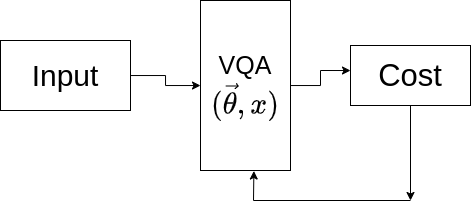
\includegraphics[width=0.3\textwidth]{./basic_vqa.png}
  \caption{}
  \label{fig:basic_vqa}
\end{wrapfigure}

\paragraph{} Parametrized circuits are quantum circuits that contain gates, depending on a certain(s) external parameters. 
For example the $\widehat{R_y}$ gate, as described in \autoref{table:basic_notions}.
These parameters will play the role of these adjustable parameters during machine learning. For example, consider a simple 
linear regression. The parameters of the quantum circuits are analogous to the weights learned during a simple linear 
regression.

The classical VQA follows the basic scheme shown in \autoref{fig:basic_vqa}.

The idea of a VQA is to find a ground state of a Hamiltonian. That is, one recalls one important 
theorems from quantum mechanics - the Variational principle. 
\begin{equation}
  E_0 \leq \frac{\bra{\psi}H\ket{\psi}}{\bra{\psi}\ket{\psi}}
  \label{eq:basic_variational_principle}
\end{equation}
meaning that this inequality is true for any states. Physically speaking, this theorem is quite trivial, 
namely, the ground state has always the smallest energy. The idea of the VQA is therefore to associate a 
Hamiltonian to the problem and to find the state that will minimize the \autoref{eq:basic_variational_principle}.
The cost function will therefore be a funciton of the form 
$\text{Cost}(\theta) = C(\theta) = \bra{\psi}H\ket{\psi}$.
One defines the following theorem (as per \cite{schuld_machine_2018}):
\begin{prettytheorem}[Deterministic quantum model]
  Let $\mathcal{X}$ be the dataset and $U(x,\theta)$ the circuit depending on the data input and the parameters, with $x\in \mathcal{X}$, and $\mathcal{M}$ 
  an observable, e.g. the Hamiltonian. Let $\ket{\psi(x, \theta) \coloneq U(x, \theta)\ket{\psi_0}}$. Then one defines a deterministic 
  quatum model as $f_{\theta} = \bra{\psi(x, \theta)}\mathcal{M}\ket{\psi(x,\theta)}$.
  \label{th:deterministic_quantum_model}
\end{prettytheorem}
This is quite an abstract and general definition. That is, in a general ML algorithm, there exists a target, that one wants to approach. In the case of the 
most general quantum algorithm, it is illustrated by the observable $\mathcal{M}$. The estimation of it is done through the application of the operator $U$ on the input 
state $\ket{\psi}$. One can say that the observable $\mathcal{M}$ is an analogy to the Hamiltonian $H$ discussed before\footnote{Even though the Hamiltonian is \underline{not an observable}.}
Before moving to a concrete example of a Variational algorithm, one defines another (2) theorem(s).
\begin{prettytheorem}[General parametrized circuit]
  A parametrized quantum circuit can be thought of as a unitary operator $U(x,\theta)$. This unitary operator 
  $U(x,\theta)$ can be represented as a sum of a purely parametrized and purely encoding circuits. That is, 
  \begin{equation}
    U(x,\theta) = W_{N+1}\prod_{i=1}^{N}S_i(x_i)W_i(\theta_i)
  \end{equation}
  depicted in circuit \ref{cirq:parametrized_embedded}. In addition, the encoding operator involved in 
  the unitary parametrized 
  operator, encoding a feature $k$ can be written as 
  \begin{equation}
    S_i(x) \equiv S(x_i) \equiv S_i(x_i) = e^{-ix_i\hat{G}_i}
  \end{equation}
  where the operator $G_i \equiv G$ is supposed to be diagonal: $G = \sum_k g_k\ket{g_k}\bra{g_k}$.
  If not, one can always change of basis making use of $P^{\dag}GP$, so that the change of base operators 
  $P^{\dag}$ and $P$ are absorbed into the encoding gates $S_i$.
  \label{th:u_as_s_and_w}
\end{prettytheorem}
\begin{wraptable}[8]{R}{9cm}
  \centering
  \begin{tblr}{c}
    \Qcircuit @C=0.75em @R=1.0em {
      \lstick{\ket{0}} &\qw & \multigate{2}{S_1}  & \qw & \multigate{2}{W_1} &      &\qw&   \multigate{2}{S_{N}} & \multigate{2}{W_{N+1}}   \\
      \vdots           &    & \ghost{S_1}         & \qw & \ghost{W_1}        &\vdots&   &   \ghost{S_{N}}     & \ghost{W_{N+1}}   \\
      \lstick{\ket{0}} &\qw & \ghost{S_1}         & \qw & \ghost{W_1}        &      &\qw&   \ghost{S_{N}}     & \ghost{W_{N+1}}   
  }
\end{tblr}
\caption{}
\label{cirq:parametrized_embedded}
\end{wraptable}

The next theorem is a bit more complex and more mathematical \cite{schuld_machine_2018}. 
This theorem makes a more explicit the expression 
given in \autoref{th:deterministic_quantum_model}. 

\begin{prettytheorem}[Deterministic quantum model (V. 2.0)]
  Let $f_\theta$ be the deterministic quantum model as defined before. Let $U(x,\theta)$ - the parametrized unitary operator 
  as defined above. The features from the $\mathcal{X}$ are also encoded as above. Then, the model is given by 
  \begin{equation}
    f_{\theta}(\vec{x}) = \sum_{\omega_{1}\in \Omega_1} \hdots \sum_{\omega_1 \in \Omega_N} c_{\omega_1 \hdots \omega_N} 
    e^{i\omega_1x_1} \hdots e^{i\omega_Nx_N} 
  \end{equation}
  where the frequency difference $\Omega_i$ is defined to be 
  \begin{equation}
    \Omega_i = \{\lambda_k - \lambda_j \; \big\vert \; k,j\in\{1,...,D\}\}
  \end{equation}
  with $D$ - the dimension of the feature space that the operator $S_i$ maps to.\footnote{
    The sketch of the proof is provided in \cite{schuld_machine_2018}.
  }
  \label{th:deterministic_quantum_model_v2}
\end{prettytheorem}

\paragraph{} In order to get this more straight, one considers the simplest case of the VQA - the variational quantum classifier, 
using the theorems and the concepts we've provied up to now.
We will consider 2 approaches to the variational quantum classifier - first one, considering the usual, plain considerations;
and the second one, using the theorem, that involves the spectrum.

The problem in question is the deterministic quantum model determined with only one encoding circuit $S_{i=1}$ 
and one qubit (one qubit variational quantum classifier).
One takes from \autoref{th:deterministic_quantum_model} $\mathcal{M}$ as $\widehat{\sigma}_z$. Taking the fact that 
$\ket{\psi(x, \theta)} = U(x, \theta)\ket{\psi_0}$, one gets thet the quantum model is given by 
\begin{equation}
  f_\theta(\vec{x}) = \bra{\psi(x,\theta)} \widehat{\sigma_z} \ket{\psi(x,\theta)} = 
  \bra{0}U^{\dag}(x,\theta)\widehat{\sigma_z}U(x,\theta)\ket{0}
\end{equation}

\paragraph{First approach} 
The ansatz of unitary $U(x,\theta)$, is given by 
\begin{equation*}
  U(x, \theta) = \text{Rot}(\theta_1, \theta_2, \theta_3)R_x(x)
\end{equation*}
The deterministic quantum model is, according to definition 
  \begin{align}
  f_\theta(x) = \bra{\psi(x, \theta)}\mathcal{M}\ket{\psi(x, \theta)} = \bra{0}U(x,\theta)^\dag \mathcal{M} U(x,\theta)\ket{0} = \\
  = \bra{0} R_x(x) \text{Rot}(\theta_1, \theta_2, \theta_3)^\dag \widehat{\sigma_z} \text{Rot}(\theta_1, \theta_2, \theta_3)R_x(x) 
  \ket{0} 
  \end{align}
  So one needs to perform a long tideous operation with matrix multiplications involved. The result is given by 
  \begin{equation}
    f_\theta(x) = \cos(\theta_2)\cos(x) - \sin(\theta_1)\sin(\theta_2)\sin(x)
  \end{equation}

Now, one defines the operator $U(x,\theta)$. The choice is more like an arbitrary choice/ansatz. 
Namely, one writes the latter operator in the form given in \ref{th:u_as_s_and_w} 
$U(x, \theta) = W_2(\theta)S_1(x)W_1(\theta)$, where the ansatz-ed operators are defined by 
$W_2(\theta) \coloneq \mathbbm{1}$, $S_1(x) \coloneq R_x(x)$ and 
$W_1(\theta) \coloneq \text{Rot}(\theta_1, \theta_2, \theta_2)$. Since $S_1 \equiv R_x(x)$ and 
$R_x = e^{-i\frac{x}{2}\sigma_x}$, thus, using the representation described in \ref{th:u_as_s_and_w}, 
$G \equiv \nicefrac{\sigma_x}{2}$. One have, however, required $G_i$ to be diagonal. One can, however, 
rewrite the Pauli operator $\sigma_x = V \sigma_z V^\dag$, so that the operator $G_i$ can 
be written in the form of $G_i = V \sigma_z V^\dag$, with $\sigma_z$ being diagonal. 
One can therefore \textit{absorb} these operators $V$, so that the argument in the exponent $e^{-iG}$ 
is diagonal. Using these representations, one can finally write:
\begin{equation}
  \begin{gathered}
    f_\theta(x) = \bra{\psi(\theta, x)}\mathcal{M}\ket{\psi(\theta, x)} \xrightarrow{\mathcal{M} = \sigma_z} \\
    \bra{\psi(\theta, x)}\sigma_z\ket{\psi(\theta, x)} \xrightarrow{\ket{\psi(x,\theta)} = U(\theta, x)\ket{0}}  
    \bra{0} U(x,\theta)^{\dag} \sigma_z U(x, \theta) \ket{0} = \\
    = \bra{0}\widehat{\text{Rot}}^\dag R_x^\dag \sigma_z R_x \widehat{\text{Rot}} \ket{0} = 
    \bra{0}\widehat{\text{Rot}}^\dag (e^{-i\frac{x}{2}\sigma_x})^\dag \sigma_z e^{-i\frac{x}{2}\sigma_x} \widehat{\text{Rot}} \ket{0} =
    \\ 
    =\bra{0}\widehat{\text{Rot}}^\dag (e^{-ixV\sigma_z V^\dag })^\dag \sigma_z e^{-ixV\sigma_z V^\dag } \widehat{\text{Rot}} \ket{0} =\\
    =\bra{0}\widehat{\text{Rot}}^\dag (Ve^{-ix\sigma_z }V^\dag)^\dag \sigma_z Ve^{-ix\sigma_z}V^\dag \widehat{\text{Rot}} \ket{0} =
    \bra{0}\widehat{\text{Rot}}^\dag Ve^{ix\sigma_z }V^\dag \sigma_z Ve^{-ix\sigma_z}V^\dag \widehat{\text{Rot}} \ket{0} =\\
  \end{gathered}
  \label{eq:variational_classifier_single_qubit}
\end{equation}
The operators $V$ and $V^\dag$ can therefore be absorbed into the observable $\mathcal{M}=\sigma_z$.
One can now use the theorem \ref{th:deterministic_quantum_model_v2}. And identify the elements 
mentioned in the theorem to those given in \autoref{eq:variational_classifier_single_qubit}.
From that, one sees that 
\begin{equation*}
  \begin{gathered*}
    N=1  \text{ , } \quad \lambda_i \in \{ -\nicefrac{1}{2}, \nicefrac{1}{2} \} \text{ ,} \quad \Omega_1 \equiv \Omega = \{-1, 0, 1\}
  \end{gathered*}
\end{equation*}

One therefore finds the value of the deterministic model
\begin{equation}
  f_\theta(x) = \sum_{\omega_i \in \Omega} c_{\omega_i} e^{i\omega_ix} = 
  c_0 + 2 \real(c_1)\cos(x) + \imaginary(c_2)\sin(x)
\end{equation}
which bizarrely resembles to the fourier series. In addition to that, one observes the 
same form of the obtained result as in the firs method of evaluating the quantum model.

\subsection*{Implementation of basic 1 qubit classifier}
One can now try to implement the basic 1 qubit variational classifier.
For that, one computes the first need to create a dataset. Namely, 
one will create the following dataset:
\begin{minted}[frame=single, linenos=true]{python}
X = np.array([0.2, 0.89, 0.121, 0.56])
Y = np.array([0, 1, 0, 1])
\end{minted}

The \texttt{X} data is the parameter of the $R_x$. What it means is that the gate $R_x$ will \textit{interpret}
the features. An example of it could be that $x$ is e.g. a footbal's team successful passes' percentage and $y$, 
whether the team has won the game.
One defines the ansatz, to be as described above, namely, $U(x,\theta)=\text{Rot}(\theta)R_x(x)$. 
One uses PennyLane to perform the operations:

\begin{listing}[ht!]
  \begin{minted}[frame=single, linenos=true]{python}
    # Define the quantum device
    dev = qml.device("default.qubit", wires=1)
    # Define the ansatz (U(x, theta))
    def ansatz(x, theta):
        qml.Rot(*theta, wires=0)
        qml.RX(x, wires=0)
    # Define the quantum node
    @qml.qnode(dev)
    def circuit(x, theta):
        ansatz(x, theta)
        return qml.expval(qml.PauliZ(0))
    # Define the cost function for the classifier
    def cost(params, X, Y):
        predictions = np.array([circuit(x, params) for x in X])
        return np.mean((predictions - Y) ** 2)
    params = np.random.uniform(size=(3,))
    # Train the classifier
    opt = qml.GradientDescentOptimizer(stepsize=0.1)
    for i in range(100):
        params = opt.step(lambda p: cost(p, X, Y), params)

  \end{minted}
\end{listing}

Let's consider what does this model do. It starts with initializing the default 1 qubit 
circuit. Then, the ansatz is initialized as discussed below. The \texttt{circuit()} evaluates the 
ansatz with inputs \texttt{x} and \texttt{theta}. The \texttt{cost()} funciton, evaluates the error 
between the obtained value of the cirquit with parameters \texttt{theta} and \texttt{x}, and the 
the target value \texttt{y}.
Then, based on that, the gradient is computed (with respect to $\theta$'s) and $\theta$'s are modified accordingly.
In other words, the $X$ are the features that are tried to be learned and adjusted, together with $\theta$'s. 
The $\theta$'s are thus trying to be adjusted so that the function $f_\theta(x) = y$ are the closest to $y$, which is the 
measured Pauli $\widehat{\sigma}_z$.

\begin{wrapfigure}{r}{0.5\textwidth}
  \centering
  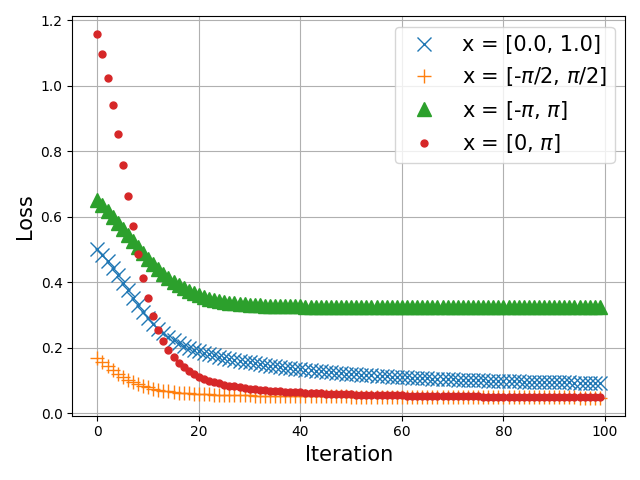
\includegraphics[width=0.5\textwidth]{loss_different_intervals.png}
  \caption{}
  \label{fig:loss_evolution}
\end{wrapfigure}
There are couple of notion that should be mentioned here. First of all, is the input data. 
The data is in form of floats in an interval of $[0,1]$. However, we're working with rotations. So, intuitively, 
there will be some kind of $\sin$, $\cos$ operations involved. Therefore, once again intuitively, the possibly 
desired interval we would want for the input data would be $[0, \pi]$ for $\cos$ 
(since $\cos$ goes over the whole range in this exact interval) and $[-\frac{\pi}{2}, \frac{\pi}{2}]$ for $\sin$ 
(since $\sin$ goes over its whole range in this excat interval).
Thus, we can compare how the loss function evolves with the number of iterations for different possible input intervals. 
This is illustrated in \autoref{fig:loss_evolution}.

Another aspect to discuss is the how is the gradient performed. Namely, in the most general case, the 
updaate mechanism of the parameters $\theta$'s is given by 
\begin{equation}
  \theta_i^{t+1} = \theta_i^{t} - \eta \frac{\partial f_\theta(x)}{\partial \theta_i^{k}}
\end{equation}
One must therefore find a way to estimate the derivative. One way is, of course use the finite differences. 
However, for quantum circuits, there is an another way of finding the derivatives.



















\newpage
\bibliographystyle{plainurl}
\printbibliography



\end{document}
